%======================================================================
%   Zak Webb
%   Ph. D. Thesis
%   Department of Physics and Astronomy
%   University of Waterloo
% 
%   Scattering on Graphs
%======================================================================


\documentclass[../thesis-main/thesis-main]{subfiles}
\begin{document}

\chapter{Scattering on graphs}

\todo{write a better introduction, including more citations}

Scattering is one of the more basic ideas of physics, with a surprisingly large usefulness.  The old joke about physicists throwing two frogs at each other \todo{cite} in order to understand their internal components has a grain of truth; particle accelerators \todo{cite}, gravitational lensing \todo{cite}, and x-ray crystallography \todo{cite} are just some examples out of many in which scattering plays a key role in physicists probing of the universe.

Along these lines, we would wonder at the usefulness of scattering in quantum information.  High energy physics uses scattering to probe atoms and molecules \todo{cite multiple}, but we would want to discretize the system for use in quantum information \todo{should I include some bit about discretized quantum field theories? Probably not}.  In this manner, we would replace the continuum by a discrete set of positions, and understand the evolution in such a model.

With this discretization, we are analyzing a system propagating on an infinite graph, and thus we can also think of this as the limit of a continuous time quantum walk to infinite graphs.  We know that quantum walks are useful algorithmic devices \todo{cite QW algorithms}, and one might wonder whether these infinite systems can allow for intuitive algorithms.  It turns out that this answer is yes, and the original motivation for graph scattering was an algorithm using graph scattering to solve a problem on boolean formulas faster than any randomized classical computation \cite{FGG08}.  This algorithm was easily understood using the intuition from scattering, and thus graph scattering became a useful tool for understanding quantum walk algorithms.

This chapter should serve as a broad introduction to graph scattering.  In particular, the notations of scattering matrices, bound states, and wavepackets have all been used in previous works.  This chapter attempts to standardize notations, while also explaining how everything works.  While there is some original work in this chapter, we also utilize and state several of the results from \cite{FGG08,Chi09,CS11,CG12} in which the author did not contribute.

\section{Free particles in the continuum}

Let us first take a look at one of the most simple quantum systems seen in any quantum mechanics text (e.g., \cite{GriQM} or \cite{SakMQM}): a free particle in one dimension.  Without any potential or interactions, we have that the time independent Schr\"{o}dinger equation reads
\begin{equation}
  \frac{\partial^2}{\partial x^2} \psi(x) = -\frac{2m}{\hbar^2}E \psi(x) = -k^2 \psi(x),
\end{equation}
which requires the (unnormalizable) solutions,
\begin{equation}
  \psi(x) = A \exp(- i k x) + B \exp(i k x) \label{eq:simple_motivating_momentum_states}
\end{equation}
for real $k$ and for arbitrary constant $A$ and $B$.  These \textit{momentum states} correspond to particles travelling with momentum $k$ along the real line, and form a basis for the entire Hilbert space.

While these momentum states are useful for understanding the propagation of particles in the quantum setting, if we want to understand more complicated behavior we need to change the potential energy of the system.  In particular, we will now include some finite-range potential $V$ that is non-zero only for $|x| < d$ for some constant $d$, so that outside this range the eigenstates remain unchanged.  The only difference is that we will deal with a superposition of states for each energy instead of the pure momentum states, forcing some relation between the $A$ and $B$ of equation \eq{simple_motivating_momentum_states}.  Namely, the eigenstates of this system become
\begin{equation}
  \psi(x) = \begin{cases}
    \exp(-i k x) + R(k) \exp(i k x) & x \leq -d\\
    T(k) \exp(- i k x) & x \geq d\\
    \phi(x,k) & |x| \leq d
    \end{cases}
\end{equation}
for some functions $R(k)$, $T(k)$, and $\phi(x,k)$ that depends on the interaction $V$.  As intuition, these states can be seen as a particle with momentum $k$ coming in from the left, hitting the potential, and then scattering (which motivates the $T$ and $R$ labels).  

In addition to these scattering states, it is also possible for bound states to exist.  These are normalizable states that have most (or all) of their amplitude near the non-zero potential, so that they do not affect scattering states that originate far from the interaction.  They simply exist as additional states in the Hilbert space.


\todo{possibly include a $\delta$-function potential scattering problem in the thesis}


\subsection{Free particles on an infinite path}

With the simple free-particle example in mind, let us now examine the discretized system.  Namely, instead of allowing arbitrary real positions, let us restrict attention to some regular 1-D lattice, such as the natural numbers.  Further, much as there is a natural linear ordering on the positions in the continuum, and in order for a particle to move between $a$ and $b$ it must travel over all positions between $a$ and $b$, in the discretized system we only allow particles to move between adjacent integers.  Explicitly, the position basis for this discretized Hilbert space will be labeled by $n\in \NN$, with transport only allowed between integers that differ by one.

If we then want to understand how this discretized system works, it will be useful to discretize the entire Schr\"{o}dinger equation.  Along those lines, remember that the second derivative of a function $f$ at $x$ can be written as
\begin{align}
  \frac{d^2}{dx^2} f(x) = \lim_{h\rightarrow 0} \frac{f(x+h) - 2 f(x) - f(x-h)}{h^2}.
\end{align}
Since we were originally working in the continuum, we could let $h$ go to zero without any problems.  In our discretize world, however, there exists some smallest difference in $x$, namely 1.  As such, we have that in our discretized space, the operator corresponding to the second position derivative can be written as
\begin{equation}
  \Delta^2 = \sum_{x=-\infty}^\infty \ket{x} \big(\bra{x-1} - 2 \bra{x} + \bra{x+1}\big) = \sum_{x=-\infty}^\infty \big(\ketbra{x}{x-1} + \ketbra{x}{x+1}\big) - 2 \II.
\label{eq:discrete_second_derivative}
\end{equation}
If we then rescale the energy levels, we have that the identity term in the right hand side of \eq{discrete_second_derivative} can be removed, so that $\Delta^2$ on this discretized one-dimensional system is proportional to the adjacency matrix of an infinite path.  

With this representation of the second derivative operator, we can see that when discretized, the time-independent Schr\"{o}dinger equation for a free particle becomes
\begin{equation}
  \Delta^2 \ket{\psi} = \Big(\sum_{x=-\infty}^\infty \big(\ketbra{x+1}{x} + \ketbra{x-1}{x}\big) - 2 \II\Big) \ket{\psi} = E'_{\psi} \ket{\psi}.
\end{equation}
If we rescale the energy term, and then break the vector equation into its components, we find that
\begin{equation}
  \braket{x+1}{\psi} + \braket{x-1}{\psi} = E_\psi \braket{x}{\psi}
\end{equation}
for all $x\in \ZZ$.  Taking motivation from the continuous case,  we then make the ansatz that $\braket{x}{\psi} = e^{i k x}$ for some $k$, and find
\begin{align}
  \braket{x+1}{\psi} + \braket{x-1}{\psi} = e^{i k } e^{i k x} + e^{-ik} e^{ikx} &= E_\psi e^{ik x} = E_\psi \braket{x}{\psi} &\Rightarrow \\ E_\psi &= e^{ik} + e^{-i k} = 2 \cos(k).
\end{align}
If we then use the fact that $E_\psi$ must be real, and that the amplitudes should not diverge to infinity as $x\rightarrow \pm \infty$, we find that the only possible values of $k$ are between $[-\pi,\pi)$.    Hence, in analogy with the continuous case, the eigenbasis of the Hamiltonian corresponds to momentum states, but where the possible momenta only range over $[-\pi,\pi)$.  We represent this momentum state with momenta $k$ as $\ket{\tilde{k}}$.

Additionally, we can discuss the ``speed'' of these eigenstates, which is given by the derivative of the energy with respect to momentum.  We con then see that 
\begin{equation}
  s = \Big| \frac{d E_k}{d k} \Big| = 2 \sin (|k|),
\end{equation}
which is to be compared with $s \propto |k|$ for in the continuum case.  While the discretization does change the relationship between momentum, energy, and speed, if we restrict ourselves to small $k$ (so that the discretization is not noticeable), we recover the linear relationship.  In this way, as the distance between vertices grows smaller, we recover the continuum case.  

One slight problem with this discussion is that these momentum states are not normalizable, and thus technically are not states in the Hilbert space.  This problem is identical to that of the continuum, and thus we shall not worry about these states of the extended Hilbert space.  However, one problem that is unique to our discretized system is that  there are an uncountable number of momentum states, while the position basis contains only a countable number of basis states.  It turns out that the resolution to this conundrum is that the two bases have different orthogonality conditions: the position basis elements are Kronecker delta orthogonal, while the momentum basis elements are Dirac $\delta$-function orthogonal.  Namely,
\begin{equation}
  \braket{\tilde{k}}{\tilde{p}} = \sum_{x=-\infty}^\infty e^{- i k x} e^{i k p} = \sum_{x=-\infty}^\infty e^{i (p-k) x} = 2\pi \delta(p-k),
\end{equation}
so that we can decompose the identity on this space as 
\begin{equation}
\II = \sum_{x=-\infty}^\infty \ketbra{x}{x} = \frac{1}{2\pi} \int_{-\pi}^\pi dk \ketbra{\tilde{k}}{\tilde{k}}.
\end{equation}


%%%%%%%%%%%%%%%%%%%%%%%%%%%%%%%%%%%%%%%%%%%%%%%
\section{Graph scattering}

Essentially, at this point we have recovered many of the results of the continuous free particle, but with a discretized position space.  The main idea behind the discretization was the change in the second derivative operator, and noting that it became proportional to the adjacency matrix of a simple graph.  This seems very similar to the case of continuous time quantum walks, in which the Hamiltonian is explicitly taken to be the adjacency matrix of a (finite sized) graph. 

As such, let us assume that the Hamiltonian of the entire system is proportional to the adjacency matrix for these graph scattering problems.  If we now want to add some finite potential to the system, in an attempt to discretize the scattering formalism, we could add a potential function, with explicit potential energies at various vertices of the infinite path.  However, if we wish to examine scattering only on unweighted graphs, we need to be a little more clever.  

To solve this problem, we will connect graphs in such a way that far from our connections the graphs will look identical to that of an infinite path, but near our changes the graph can differ drastically from an infinite path.  In particular, we will use an arbitrary (finite) graph as a base, and connect semi-infinite (infinite in one direction) paths to this base graph.

With this construction, the eigenvalue equation must still be satisfied along the semi-infinite paths, and thus the form of the eigenstates along the paths must still be of the form $e^{i k x}$ for some $k$ and $x$.  However, we can no longer assume that $k$ is real, as the fact that the attached semi-infinite paths are only infinite in one direction allow for an exponentially decaying amplitudes along the paths.  Additionally, we can have nontrivial correlations between the amplitudes among the different paths, similar to the correlated reflection and transmission coefficients in the continuous case.

Note that the topic of graph scattering is widely used in the literature.  Most of this section is not original work, and should be taken as background material.  In particular, these results are taken from \cite{FGG08, Chi09, CS11, CG12}

\todo{Find more accurate citations}

%%%%%%%%%%%%%%%%%%%%%%%%%%%%%%%%%%%%%%%%%%%%%%%
\subsection{Infinite path and a Graph}\label{sec:infinite_path_and_graph}

In the most simple example, let us attached a graph $\widetilde{G}$ to an infinite path.  In particular, we assume that $\widetilde{G}$ is attached to a single vertex of the infinite path, and that the graph is attached by adding an edge from each vertex in $S\subset V(\widetilde{G})$ to one specific vertex of the infinite path, which we label $0$, as seen in \fig{path_and_graph}.  Calling this new graph $G$, the adjacency matrix of $G$, and thus the Hamiltonian for this scattering problem, can be seen to be
\begin{equation}
  A(G) = A(\widetilde{G}) + \sum_{v\in S \subset V(\widetilde{G})} \ketbra{v}{0} + \ketbra{0}{v} + \sum_{x=-\infty}^\infty \ketbra{x}{x+1} + \ketbra{x+1}{x}.
\end{equation}

If we then want to inspect the eigenvectors of this Hamiltonian, we find that the eigenvalue equation on the infinite path is identical to that of an infinite path without the graph attached.  Hence, we can see that any eigenstate of the Hamiltonian must take the form $Ae^{i k x} + Be^{-i k x}$ for some $k$ along the infinite paths.  


%%%%%%%%
\begin{figure}
  \centering
  \tikzsetnextfilename{GS_path_and_graph}
  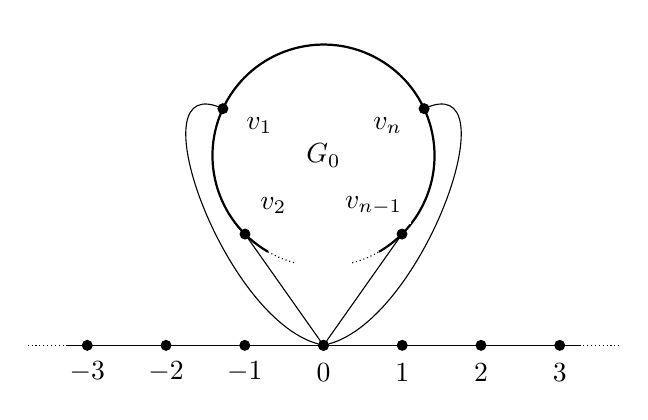
\begin{tikzpicture}[
  label distance=-5.5pt,
  thin,
  vertex/.style={circle,draw=black,fill=black,inner sep=1.25pt,
    minimum size =0mm},
  attach/.style={circle,draw=black,fill=white,inner sep=1.25pt,
    minimum size =0mm},
  dots/.style={circle,fill=black,inner sep=.5pt,
    minimum size= 0pt}]

% Path and Labels    
  \draw (-3.25,-2.41) -- (3.25,-2.41);
  
  \foreach \x in {-3,...,3}{
    \node at (\x,-2.41) [vertex] {};
    \node at (\x,-2.75) {$\x$};
  }
    
  \node (a) at (0,-2.41) [vertex] {};
  
  \draw[densely dotted] (-3.25,-2.41) -- (-3.75, -2.41);
  \draw[densely dotted] (3.25, -2.41) -- (3.75, -2.41);
  
% Graph  
  \draw[thick] (240:1.41) arc (240:-60:1.41);
  \draw[densely dotted] (240:1.41)  arc (240:255:1.41);
  \draw[densely dotted] (285:1.41)  arc (285:300:1.41);
  
  \foreach \i / \n /\t in {25 / n/ 15, 155 / 1/ 165, 225/ 2 / 120, 315 / {n-1}/60}{
    \node at (\i : .9) [rectangle,fill=white] {$v_\n$};
    \node at (\i : 1.41) [vertex] {};
  }
  \node at (0,0) [rectangle,fill=white] {$G_0$};

% Attaching Edges
  \foreach \i /\t in {25/15, 155/165}{
    \draw (\i:1.41) to[out=\i,in=\t] (a);
  }
  
  \foreach \i \in in {225,315}{
    \draw (\i:1.41) to (a);
  }

\end{tikzpicture}
  \caption{A simple example for graph scattering.  A graph $\widetilde{G}$ is attached to an infinite path.}
  \label{fig:path_and_graph}
\end{figure}

With this assumption, we can see that there are three distinct cases for the form of the eigenstates.  In particular, the eigenstate could have no amplitude along the infinite paths, being confined to the finite graph $\widehat{G}$.  It could also be a normalizable state not confined to the finite graph $\widehat{G}$, in that the amplitude along the infinite paths decays exponentially.  Finally, the eigenstate could be an unnormalizable state, in which case we will call it a scattering state.

In the first case, where the state is confined to the graph $\widetilde{G}$, we have the major restriction that the state $\ket{\psi}$ satisfies 
\begin{align}
  \braket{x}{\psi} = 0
\end{align}
for all $x\in \NN$.  Additionally, if $\ket{\phi}$ is the restriction of $\ket{\phi}$ to the finite graph $\widetilde{G}$, we have that 
\begin{align}
  A(\widetilde{G}) \ket{\phi} = E \ket{\phi}
\end{align}
so that $\ket{\phi}$ is an eigenstate of the graph $\widetilde{G}$, that also satisfies
\begin{align}
  \sum_{v\in S} \braket{v}{\phi} = 0.
\end{align}
These restrictions together show that these completely bound states have an extremely restricted form as eigenstates of $A(\widetilde{G})$, but the infinite path does not really affect them.  In particular, their energies are not restricted by anything other than the graph itself, but we are guaranteed to have at most $|V(\widetilde{G})|$ of these confined bound states.

In the second case, we could have that the eigenstate is normalizable, but is not confined to the graph $\widetilde{G}$.  In this case, we have that the amplitudes along the infinite paths must go to zero, but they must still be a sum of exponentials.  As such, we have that $\ket{\psi}$ must be of the form
\begin{align}
  \braket{x}{\psi} = A z^x
\end{align} 
for some $z\in (-1,1)\setminus \{0\}$ for all $x\in \NN$, so that the energy must be $z+ z^{-1}$ (the case for $z= 0$ forces $A = 0$, and we are in the first case).  Additionally, we can see that if $\ket{\phi}$ is the restriction of $\ket{\psi}$ to those vertices inside the graph $A(\widetilde{G})$, they must satisfy
\begin{align}
  A(\widetilde{G}) + A \sum_{v\in S} \ket{v}\braket{v}{\phi} = 2 \cos (k) \ket{\phi},
\end{align}
a modified version of the eigenvalue equation for the graph $A(\widetilde{G})$.

Let us finally assume that the state is a scattering state.  Note that the eigenvalue of the state must be in the range $[-2,2]$, and that the form of the eigenstate along the paths must be scalar multiples of $e^{ikx}$ and $e^{-ikx}$, for some $k\in [-\pi, \pi]$.  Explicitly, the state must be of the form
\begin{align}
  \braket{x}{\psi} = \begin{cases} Ae^{i k x} + B e^{i k x} & x \leq 0\\
   C e^{i k x} + D e^{i k x} & x\geq 0\end{cases}
\end{align}
where we note that the amplitude can change at $x=0$, since we have attached the graph $\widetilde{G}$.  However, we do have that $A + B=C +D$, since the amplitude at $0$ is single valued, and that the eigenvalue of this state is given by $2\cos(k)$.  Note that we have not yet determined the form of the eigenstate inside the graph $\widetilde{G}$, but if we define $\ket{\phi}$ to be the restriction of $\ket{\psi}$ to the finite graph $\widetilde{G}$, then $\ket{\phi}$ must satisfy the equation
\begin{equation}
  A(G) \ket{\phi} + (A+ B)\sum_{v\in S} \ket{v}\braket{v}{\phi} = 2\cos(k) \ket{\phi},
\end{equation}
where the additional term arises from the fact that the vertices in $S$ are connected to the vertex $0$.  Finally, we have that
\begin{equation}
  2 \cos(k)\braket{0}{\psi} = Ae^{-ik} + B e^{ik} + C e^{i k} + D e^{-ik} + \sum_{v\in S} \braket{v}{\phi},
\end{equation}
since the eigenvalue equation must be satisfied at $0$.

In the first two cases, we have that the state is highly localized to the area surrounding the graph $\widetilde{G}$, and thus they do not have a large effect on wavefunctions that originate far from the graph.  However, the aptly named scattering states can be used to determine the time evolution of these wave functions.  In particular, if we look at the case where $A = 1$ and $D = 0$,  we can see that
\begin{align}
  \braket{x}{\psi} = \begin{cases} e^{-ikx} + B e^{i kx} & x\leq 0\\
  C e^{-ikx} & x \geq 0\end{cases}
\end{align}
so that $1+ B  =C$.  Note that this is reminiscent of a scattering state, with reflection amplitude $B$ and transmission amplitude $C$.  We can then take as intuition that these scattering states represent a wavepacket with momentum exactly $k$ traveling towards the graph $G$, and then scattering with these amplitudes.  We will use this intuition for our definitions of scattering on more general graphs. 
 
%%%%%%%%%%%%%%%
\subsection{General graphs}\label{sec:general_graphs}

Let us now turn our attention to scattering on more general graphs.  In particular, let $\widehat{G}$ be any finite graph, with $N+m$ vertices and an adjacency matrix given by the block matrix
\begin{equation}
  A(\widehat{G}) = \begin{pmatrix}A & B^\dag\\ B & D\end{pmatrix},
\end{equation}
where $A$ is an $N\times N$ matrix, $B$ is an $m\times N$ matrix, and $D$ is an $m\times m$ matrix.  When examining graph scattering, we will be interested in the graph $G$ given by the graph-join of $\widehat{G}$ and $N$ semi-infinite paths, with an additional edge between each of the first $N$ vertices of $\widehat{G}$ and the first vertex of one semi-infinite path.  A schematic example can be seen in \fig{basic_graph}.

We shall label call the first $N$ vertices of the graph \emph{terminal vertices}, as they connect the semi-infinite paths to the finite graph $\widehat{G}$, and we shall label them as $(1,i)$, where $i\in[N]$.  Analogously, we will refer to the vertices on the $N$ semi-infinite paths as $(x,i)$ for $x\in \NN^+$ and $i\in[N]$, with the $i$ label referring to the particular semi-infinite path on which the vertex is labeled, while the label $x$ denotes the location along the path.  We also refer to the remaining $m$ vertices of $\widehat{G}$ as the \textit{internal vertices} of $\widehat{G}$, and label them as $w\in[m]$.  With this labeling of the vertices of $G$, the adjacency matrix of $G$ is then given by
\begin{equation}
  A(G) = A(\widehat{G}) + \sum_{j=1}^N \sum_{x=1}^\infty \big(\ketbra{x,j}{x+1,j} + \ketbra{x+1,j}{x,j}\big).
\end{equation}

At this point, we want to examine the possible eigenstates of the matrix $A(G)$.  It turns out that there are 3 different kinds of eigenstates, corresponding to the different qualitative properties of the eigenstate along the semi-infinite paths, exactly as in the case studied in \sec{infinite_path_and_graph}.

While we will mostly be interested in the third such type, corresponding to scattering off of the graph, the other two kinds remain important for a decomposition of the identity.  In particular, we will be guaranteed that these three kinds of eigenstates will form an orthogonal basis for the Hilbert space, and thus we will be able to use this decomposition to guarantee particular behavior of time evolved states.

\begin{figure}
  \centering
  \tikzsetnextfilename{GS_basic_graph}
  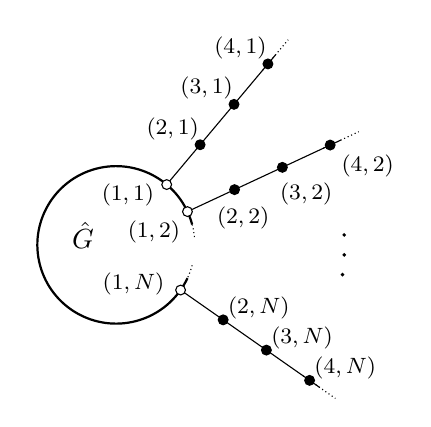
\begin{tikzpicture}[
  label distance=-5.5pt,
  thin,
  vertex/.style={circle,draw=black,fill=black,inner sep=1.25pt,
    minimum size =0mm},
  attach/.style={circle,draw=black,fill=white,inner sep=1.25pt,
    minimum size =0mm},
  dots/.style={circle,fill=black,inner sep=.5pt,
    minimum size= 0pt},
  every text node part/.style={font=\footnotesize}]

  \node at (.15, .63) [rectangle,fill=white] {$(1,1)$};
  \node at (.48, .17) [rectangle,fill=white,inner sep=0pt] {$(1,2)$};
  \node at (.22,-.5) [rectangle,fill=white] {$(1,N)$};

  \draw[thick] (15:1) arc (15:335:1);
  \draw[densely dotted] (15:1)  arc (15:5:1);
  \draw[densely dotted] (-15:1)  arc (-15:-25:1);

  \node at (-.42,.12) [rectangle] {\normalsize${\hat{G}}$};

  \foreach \x  in {50, 25,-35}{
    \draw (\x:1cm) -- (\x:3.15cm);
    \draw (\x:2.9cm) -- (\x:3.4cm) [densely dotted];
  }
  
  \node at (50:1)[attach]{};
  \node at (50:1.66)[vertex,label=150:{$(2,1)$}]{};
  \node at (50:2.33)[vertex,label=150:{$(3,1)$}]{};
  \node at (50:3)[vertex,label=150:{$(4,1)$}]{};

  \node at (25:1)[attach]{};
  \node at (25:1.66)[vertex]{};
  \node at (25:2.33)[vertex]{};
  \node at (25:3)[vertex]{};
  
  \node at (12:1.65) {$(2,2)$};
  \node at (15:2.5) {$(3,2)$};
  \node at (17.5:3.35) {$(4,2)$};

  \node at (-35:1)[attach]{};
  \node at (-35:1.66)[vertex,label=60:{$(2,N)$}]{};
  \node at (-35:2.33)[vertex,label=60:{$(3,N)$}]{};
  \node at (-35:3)[vertex,label=60:{$(4,N)$}]{};

  \node at (-2.5:2.9)[dots] {};
  \node at (2.5:2.9)[dots] {};
  \node at (-7.5:2.9)[dots] {};
\end{tikzpicture}
  \caption{An infinite graph $G$ obtained from a finite graph $\widehat{G}$ by attaching $n$ semi-infinite paths. The open circles are \emph{terminals}, vertices of $\widehat{G}$ to which semi-infinite paths are attached. The internal vertices of $\widehat{G}$ are not shown.}
  \label{fig:basic_graph}
\end{figure}


%%%%
\subsubsection{Confined bound states}

The easiest states to analyze are the confined bound states, which are eigenstates in which the only nonzero amplitudes are on vertices inside the finite graph $\widehat{G}$. If any vertex on the semi-infinite paths has nonzero amplitude for some eigenstate of the Hamiltonian, then the form of the Hamiltonian forces all vertices on that path to have nonzero amplitude, and thus these confined bound states are exactly those states that have finite support in the basis of vertex states.  

To find these confined bound states, we restrict our Hilbert space to the space spanned by the internal vertices of $\widehat{G}$. The states of interest then correspond to the eigenstates of $D$ (the induced adjacency matrix of $A(G)$ when restricted to the internal vertices of $\widehat{G}$) with the additional restriction that the state lies in the nullspace of $B^\dag$, so that we can extend this state to the full Hilbert space by simply assuming all other amplitudes are zero.    

As we originally assumed that there are only $m$ internal vertices of $\widehat{G}$, there are at most $m$ such confined bound states.  Additionally, note that there are no restrictions on the eigenvalues of these states, other than those that are inherited from any restrictions placed on it by $D$ (such as the energy being bounded by the maximum degree of $\widehat{D}$).

%%%%
\subsubsection{Unconfined bound states}

The next possible type of eigenstates are those that are not confined to the finite graph $\widehat{G}$ but are still normalizable.  Since these states still have amplitude along the semi-infinite paths, we know that they must be of the form $Ae^{i k x}$, for some $A$ and $k$.  However, when $k$ is not real (corresponding to a decaying amplitude along the paths), we have that
\begin{equation}
  2 \cos(k) = 2\cos(k_r + i k_i) = 2 \cos(k_r) \cosh(k_i) - i \sin(k_r) \sinh(k_i).
\end{equation}
Hence, if we assume that the state is normalizable, then $k_i \neq 0$, and as the adjacency matrix is Hermitian, we must have that the eigenvalue is real, forcing $k_r = \pi n$ for some $n\in \NN$.  Note that this then implies that $e^{i k} = z$, for some $z\in(-1,1)\setminus\{0\}$ (where $0$ corresponds to the confined bound states).

As the eigenvalue equation for these states are guaranteed to be satisfied along the paths, we need to construct the form of the eigenstates inside the graph $\widehat{G}$.  We can then see that the eigenvalue equation for these vertices is given by
\begin{align}
\bigg[
  \begin{pmatrix} 
    A & B^\dag\\
    B & D
  \end{pmatrix}
  + \begin{pmatrix} 
    z \\
    0
  \end{pmatrix}
  \bigg] \begin{pmatrix}
    \vec{\alpha}\\
    \vec{\beta}
  \end{pmatrix} = \Big(z + \frac{1}{z}\Big) \begin{pmatrix} 
    \vec{\alpha}\\
    \vec{\beta}
  \end{pmatrix}
\end{align}
where $\vec{\alpha} \in \CC^N$ and $\vec{\beta}\in \CC^m$.  Note that the amplitudes for a vertex $(x,i)$ is given by $\vec{\alpha}_i z^{x-1}$.  Note that we are implicitly assuming that $\vec{\alpha} \neq \vec{0}$, for in that case we are working with a confined bound state.  

While there is no immediate reason to guess that the total number of bound states is finite, it has been shown that this number is indeed finite (see \cite{CG12} for a more thorough explanation, using Levinson's theorem for graphs).

\todo{I know that they are finite from the Levinson's theorem, but is there any other reason to guarantee that they are finite?}


%%%%
\subsubsection{Scattering states}

We finally reach the point of scattering states, or those unnormalizable eigenstates of the Hamiltonian.  We first assume that these states are orthogonal to all bound states, and in particular that we are orthogonal to all confined bound states, as this allows us to uniquely construct the scattering states (without this assumption, if there existed a confined bound state at the appropriate energy, then we could simply add any multiple of the confined bound state to get a different scattering state).

Taking some intuition from the classical case, we will construct a set of states that correspond to sending a particle in towards the graph $\widehat{G}$ along one of the semi-infinite paths and understanding how it scatters off of the graph.  Namely, for each $i\in[N]$ we will assume that there exists a state with amplitude along the $i$-th path of the form $e^{i k x} + S_{i,i}(k)e^{-i k x}$ for $k\in (-\pi, 0)$, and that the rest of the paths have amplitudes given by $S_{i,q}(k)e^{ikx}$.  More concretely, we assume that the form of the states is given on the infinite paths by
\begin{equation}
  \braket{x,q}{\scat_{j}(k)} = \delta_{j,q} e^{-i k x} + S_{qj} e^{i k x}.\label{eq:scattering_amplitude_paths}
\end{equation}
We then need to see whether such an eigenstate exists.  In this case, note that $S_{qj}$ corresponds to the transmitted amplitude along the $q$-th path if the particle was incident along the $j$-th path.  In the continuous case, $S$ forms a unitary matrix, which essentially means that any incoming particle must also leave, and be distinguishable from a particle incident from a different direction.  This intuition will also hold in the discrete case, but we will show this later.

\todo{this seems a little clunkly; try to go over and rewrite}

If we continue to make the assumption that these states exist, we can also write the amplitudes of the $m$ interval vertices as a column vector, as $\vec{\psi}_i(k)$, in which $\vec{\psi}_{i}(k)$ is the projection of $\ket{\scat_j(k)}$ onto the internal vertices of $\widehat{G}$.  We can then collect these vectors into an $m\times N$ matrix, namely
\begin{equation}
  \Psi(k) := \begin{pmatrix} \vec{\psi}_1(k) & \vec{\psi}_2(k) & \cdots & \vec{\psi}_N(k)\end{pmatrix}
\end{equation}

Noting that the amplitudes for $\ket{\scat_j(k)}$ on the terminal vertices is given by $ e^{-i k}\delta_{j,q} + S_{qj}(k)e^{ik}$, we can then collect all of the eigenvalue equations for the vertices in $\widehat{G}$ (both internal and termal) as
\begin{equation}
  \begin{pmatrix} A & B^\dag \\
    B & D\end{pmatrix} \begin{pmatrix}  e^{-i k} \II + S(k) e^{i k}\\ \Psi(k)\end{pmatrix} 
    + \begin{pmatrix} e^{-2 i k} \II + e^{2 i k} S(k)\\ 0\end{pmatrix} = 
    2 \cos(k) \begin{pmatrix}  e^{-i k} \II + S(k) e^{i k}\\ \Psi(k)\end{pmatrix},
\end{equation}
where we have constructed the scattering matrix $S(k)$ using the scattering amplitudes $S_{qj}(k)$.

By examining the lower half of this matrix equation, we can see that
\begin{equation}
  \Psi(z) = \frac{1}{2 \cos(k) \II - D} \big( e^{-ik} B + e^{i k} B S(z)\big),
\end{equation}
which gives the amplitudes of the internal vertices in terms of the scattering matrix.  Note that we have assumed that the matrix $D$ does not have an eigenvalue equal to $2\cos(k)$, but this assumption will not be critical, as the eventual matrix $\ket{\Psi}(z)$ will be defined by analytic continuation.

Let us now examine the upper half of the matrix equation, to find
\begin{align}
  A\big(e^{-ik} \II+ e^{i k} S(k)\big) + B^\dag \Psi(k) + \big(e^{-2 ik}\II + e^{2 i k} S(z)\big) &= 2 \cos(k) \big(e^{-ik} \II + e^{i k} S(k)\big)\\
  -\Bigg(\II - e^{ik}\Big(A + B^\dag \frac{1}{2 \cos(k) - D} B\Big)\Bigg)S(k) &= \II - e^{-ik}\Big(A + B^\dag \frac{1}{2 \cos(k) - D} B\Big).
\end{align}
Hence, if we define
\begin{equation}
  Q(k) = \II - e^{ik}\Big( A + B^\dag \frac{1}{2 \cos(k) - D} B\Big),
\end{equation}
we find that
\begin{equation}
  S(k) = - Q(k)^{-1} Q(-k),
\end{equation}
if we assume that the matrix $Q(k)$ can be inverted.  Note that for all ${k\in (-\pi,0)}$, this might only be impossible for $k$ in which $D$ has a $2\cos(k)$ eigenvalue, in which case we have already run into a problem with the definition of $\Psi(k)$.

Putting this all together, we then have that the states $\ket{\scat_j(k)}$ exist for all $k\in (-\pi,0)$ for which $D$ does not have a $2\cos(k)$ eigenvalue.  We will see in \sec{def_of_gamma_matrix} that this restriction is an artifact of our construction of $S(k)$, and thus the scattering states will be well defined for all $k\in (-\pi,0)$.


%%%%
\subsubsection{Half-bound states}

As a limiting case for both the scattering states and the unconfined bound states, we have those states with $k = 0$ or $k= \pi$ (or equivalently with $z = \pm 1$).  In either case, the two momenta correspond to particles that don't move, but the states themselves are not normalizable.  They won't play much of a role in this paper, but I did want to mention them.


%%%%
\subsubsection{Scattering states for all $k$}\label{sec:def_of_gamma_matrix}

While the above construction is a useful definition of the scattering states for most ${k\in(-\pi,0)}$, unfortunately there are specific values of $k$ (namely those for which $D$ has eigenvalue $2\cos(k)$) in which the above analysis doesn't hold, due to the singularity of particular matrices.  If we want to show that these scattering states exist for all $k\in (-\pi,0)$, we need to somehow show that these singularities are just a problem of the analysis and are not intrinsic barriers to existence.  Note that this construction closely follows that of \cite{CG12}.

Along these lines, let us extend our analysis to complex $z$, instead of only focusing on amplitudes of the form $e^{ik}$.  We will define the matrix
\begin{equation}
  \gamma(z) := \begin{pmatrix}  z A - \II & z B^\dag\\
    z B & zD - (1+z^2) \II\end{pmatrix}.
    \label{eq:gamma_def}
\end{equation}
This matrix is closely related to the eigenvalue equation for vertices of the graph $\widehat{G}$, but with $e^{ik}$ replaced with $z$.  

With this definition, it will be useful to note the following matrix equalities.  In particular, assuming that $z$ is a complex number such that the following matrices are not singular, we have:
\begin{align}
  \begin{pmatrix} \II & zB^\dag\\
    0 & z D - (1+ z^2) \II \end{pmatrix}
    \begin{pmatrix} - Q(z) & 0\\
      \frac{z}{zD - (1+ z^2)\II}B & \II\end{pmatrix} 
      &= \begin{pmatrix} -Q(z) + z B^\dag \frac{1}{D - (z + z^{-1})} B & z B^\dag\\
        zB & zD - (1+z^2)\II\end{pmatrix} \\
        &= \gamma(z)
\end{align}
Additionally, if we note that the inverse of a block diagonal matrix can be written as
\begin{equation}
  \begin{pmatrix} X & Y \\
  Z & W\end{pmatrix}^{-1} = \begin{pmatrix} \big(X - Y W^{-1} Z\big)^{-1} & - X^{-1} Y \big(W - Z X^{-1} Y\big)^{-1}\\
    - W^{-1} Z \big(X - Y W^{-1} Z\big)^{-1} & \big(W - Z X^{-1} Y\big)^{-1}\end{pmatrix},
\end{equation}
we can then invert this equation for $\gamma(z)$ as 
\begin{align}\gamma(z)^{-1} &= \begin{pmatrix} - Q(z) & 0\\
      \frac{z}{zD - (1+ z^2)\II}B & \II\end{pmatrix}^{-1} \begin{pmatrix} \II & zB^\dag\\
    0 & z D - (1+ z^2) \II \end{pmatrix}^{-1}\\
    &= \begin{pmatrix}
      - Q(z)^{-1} & 0\\
      \frac{z}{z D - (1+z^2)\II} B Q(z)^{-1} & \II
    \end{pmatrix}
    \begin{pmatrix}
      \II & - B^{\dag} \frac{z}{zD - (1+z^2)\II}\\
      0 & \frac{1}{zD - (1+z^2)\II}
    \end{pmatrix}.
\end{align}
Combining these two matrix equations, we can then find that
\begin{align}
  \gamma (z)^{-1} \gamma(z^{-1}) &= \begin{pmatrix}
      - Q(z)^{-1} & 0\\
      \frac{z}{z D - (1+z^2)\II} B Q(z)^{-1} & \II
    \end{pmatrix}
    \begin{pmatrix}
      \II & - B^{\dag} \frac{z}{zD - (1+z^2)\II}\\
      0 & \frac{1}{zD - (1+z^2)\II}
    \end{pmatrix}\nonumber\\
  &\qquad \qquad \times
    \begin{pmatrix} \II & z^{-1}B^\dag\\
    0 & z^{-1} D - (1+ z^{-2}) \II \end{pmatrix}
    \begin{pmatrix} - Q\big(z^{-1}\big) & 0\\
      \frac{z^{-1}}{z^{-1}D - (1+ z^{-2})\II}B & \II\end{pmatrix} \\
  &=  \begin{pmatrix}
      - Q(z)^{-1} & 0\\
      \frac{z}{z D - (1+z^2)\II} B Q(z)^{-1} & \II
    \end{pmatrix}
    \begin{pmatrix}
      \II & 0\\
      0 &z^{-2}\II \end{pmatrix}
    \begin{pmatrix} - Q\big(z^{-1}\big) & 0\\
      \frac{z^{-1}}{z^{-1}D - (1+ z^{-2})\II}B & \II\end{pmatrix} \\
   &= \begin{pmatrix}
      - Q(z)^{-1} & 0\\
      \frac{z}{z D - (1+z^2)\II} B Q(z)^{-1} &z^{-2} \II
    \end{pmatrix}
    \begin{pmatrix} - Q\big(z^{-1}\big) & 0\\
      \frac{z^{-1}}{z^{-1}D - (1+ z^{-2})\II}B & \II\end{pmatrix} \\
  &= \begin{pmatrix}
      Q(z)^{-1}Q(z^{-1}) & 0\\
      \frac{1}{D - (z+z^{-1})\II }B \big(z^{-2} \II - Q(z)^{-1}Q(z^{-1}) \big) & z^{-2}\II
    \end{pmatrix}\\
  &= -\begin{pmatrix}
      S(z) & 0\\
     z^{-1} \Psi(s) & -z^{-2}\II
    \end{pmatrix},\label{eq:gamma_gives_S}
\end{align}
where we have extended the definition of $S$ and $\Psi$ to all complex $z$ instead of just $e^{ik}$

With these matrix equations, we have a representation of the scattering matrix and the interior amplitudes in terms of the matrix $\gamma$.  If we then note that
\begin{equation}
  \gamma(z)^{-1} = \frac{1}{\det \gamma(z)} \adj \gamma (z)
\end{equation}
where $\adj \gamma (z)$ is the adjugate matrix of $\gamma(z)$, then by \eq{gamma_gives_S} we can then see that the entries of $\gamma(z)$, and thus the entries of $S(z)$ and $\Psi(z)$, are rational functions of $z$. 

With this fact, to show that the problems defining the states $\ket{\scat_j(k)}$ are a result of our analysis rather than intrinsic difficulties, we need only show that there are no poles in the matrix elements for $S(z)$ or $\Psi(z)$ for $z$ on the unit circle.  We actually have that for all such $z$, there is an upper bound on the norm of the scattering amplitudes, which might depend on the graph $\widehat{G}$.
\begin{lemma}
Given $\widehat{G}$, there exists a constant $\lambda\in\mathbb{R}$ such that $|\langle v|sc_{j}(k)\rangle|<\lambda$ for all $k\in[-\pi,\pi)$, $j\in\{1,\ldots,N\}$, and $v\in\widehat{G}$.
\end{lemma}\label{lem:scattering_state_amplitude_bound}

\begin{proof}
Note that 
\begin{equation}
\gamma\left(\frac{1}{z}\right)=\frac{1}{z^{2}}\gamma(z)+\left(\frac{1}{z^{2}}-1\right)\widehat{P}\end{equation}
where 
\begin{equation}
\widehat{P}=\begin{pmatrix}
1 & 0\\
0 & 0\end{pmatrix}
\end{equation}
projects onto the $N$ vertices of $\widehat{G}$ attached to semi-infinite paths. Hence 
\begin{equation}
-\gamma(z)^{-1}\gamma\left(\frac{1}{z}\right)=-\frac{1}{z^{2}}+\left(1-\frac{1}{z^{2}}\right)\gamma(z)^{-1}\widehat{P}.
\end{equation}

Let $\{|\psi_{c}\rangle \colon c\in\{1,\ldots,n_{c}\}\}$ be eigenstates of $\widehat{H}$ satisfying $\widehat{P}|\psi_c\rangle=0$, and let this set be an orthonormal basis for the span of all such states. Then
 \begin{equation}
\left(1-\frac{1}{z^{2}}\right)\gamma(z)^{-1}\widehat{P}=\left(1-\frac{1}{z^{2}}\right)\left(1-\sum_{j=1}^{n_{c}}|\psi_{c}\rangle\langle\psi_{c}|\right)\gamma(z)^{-1}\left(1-\sum_{j=1}^{n_{c}}|\psi_{c}\rangle\langle\psi_{c}|\right)\widehat{P}\end{equation}
 since each $|\psi_c\rangle$ is an eigenvector of $\gamma(z)$ and
$\widehat{P}|\psi_{c}\rangle=0$. Reference \cite{CG12} shows (in Part 2 of the proof of Theorem 1) that
\begin{equation}
\det\left(\frac{1}{1-z^{2}}\right)M(z)\neq0\text{ for }|z|=1,
\end{equation}
where $M(z)$ is the $(N+m-n_{c})\times(N+m-n_{c})$ matrix of $\gamma(z)$ in the subspace of states orthogonal to the span of $\{|\psi_{c}\rangle \colon c\in\{1,\ldots,n_{c}\}\}$. Therefore 
\begin{align*}
\frac{1}{z}\langle v|\mathrm{sc}_{j}(k)\rangle & =  -\langle v|\gamma(z)^{-1}\gamma\left(\frac{1}{z}\right)|j\rangle\\
 & = \langle v|\left(1-\frac{1}{z^{2}}\right)\left(1-\sum_{j=1}^{n_{c}}|\psi_{c}\rangle\langle\psi_{c}|\right)\gamma(z)^{-1}\left(1-\sum_{j=1}^{n_{c}}|\psi_{c}\rangle\langle\psi_{c}|\right)|j\rangle
\end{align*}
has no poles on the unit circle, and the result follows.

\end{proof}

As such, we have that the scattering states are well defined for all $k\in (-\pi,0)$.  


%%%%%%%%%%%%%%%
\subsection{Scattering matrix properties}

While the use of the $\gamma$ matrix gives an explicit construction of the form of the eigenstates on the internal vertices, the alternate definition in terms o the $Q$ matrix can be used to easily show several properties of the scattering matrix.  In particular, remember that
\begin{equation}
  S(k) = - Q(z)^{-1} Q(z^{-1}),
\end{equation}
where $z=e^{i k}$, and the matrices $Q(z)$ are given by
\begin{equation}
  Q(z) = \II - z \Big( A + B^\dag \frac{1}{ \frac{1}{z} + z - D} B\Big).
\end{equation}
Note that $Q(z)$ and $Q(z^{-1})$ commute for all $z\in \CC$, as they can both be written as $\II + z H(z + z^{-1})$.

Using this expression for the scattering matrix, it is easy to see that $S(k)$ is a unitary matrix, as 
\begin{equation}
  S(k)^{\dag} = - Q(z^{-1})^\dag (Q(z)^{-1})^\dag
\end{equation}
and that
\begin{equation}
  Q(z)^\dag = \II^\dag - z^\dag\Big( A^\dag + B^\dag \Big(\frac{1}{\frac{1}{z} + z - D}\Big)^\dag (B^\dag)^\dag\Big) 
     = \II - z^\dag \Big(A + B^\dag \frac{1}{\frac{1}{z^\dag} + z^\dag - D} B \Big) = Q(z^\dag)
\end{equation}
and thus
\begin{equation}
  S(k)^\dag = -Q(z^{-1})^\dag (Q(z)^{-1})^\dag = - Q(z) Q(z^{-1})^{-1} = Q(z^{-1})^{-1} Q(z) = S(k)^{-1}
\end{equation}
where we used the fact that $z=e^{ik}$ so that $z^\dag = z^{-1}$, and the fact that $Q(z)$ and $Q(z^{-1})$ commute.

Additionally, we can make use of the fact that $S$ is derived from an unweighted graph to show that the scattering matrices are symmetric.  In particular, note that $Q(z)$ is symmetric for all $z$, since $D$ is symmetric, symmetric matrices are closed under inversion, $A$ is symmetric and $B$ is a 0-1 matrix.  As such, we have that
\begin{align}
  S(k)^T &= -\big( Q(z)^{-1} Q(z^{-1})\big)^T = -Q(z^{-1})^T (Q(z)^{-1})^T \\
    &= -Q(z^{-1}) Q(z)^{-1} = -Q(z)^{-1} Q(z^{-1}) = S(k)
\end{align}
where we used the fact that $Q(z)$ and $Q(z^{-1})$ commute.

Putting this together, we have that $S(k)$ is a symmetric, unitary matrix for all $k$.

%%%%%%%%%%%%%%%%%
\subsection{Orthonormality of the scattering states}

We now have some basic ideas behind the scattering behavior.  In particular, we have that the scattering states exist for all $k$, and that the scattering matrices are symmetric and unitary.  However, one of the most important behaviors we need is that the scattering states are orthonormal, and that they form a basis for the Hilbert space corresponding to the graph. 

We will first show that two scattering states are orthonormal.

\begin{lemma}
  Let 	$k,p\in (-\pi,0)$, and let $i,j\in [N]$.  We then have that
  \begin{align}
    \braket{\scat_i(p)}{\scat_{j}(k)} = \frac{1}{2\pi} \delta_{i,j} \delta(p-k),
    \label{eq:delta}
  \end{align}
  where the two sides are equal as functionals against integration.
\label{lem:orthonormality_of_scattering_states}
\end{lemma}
\begin{proof}
Let 
\begin{align}
\Pi_{1} & = \sum_{x=1}^{\infty}\sum_{q=1}^{N}|x,q\rangle\langle x,q|%\\
&\Pi_{2} & = \mathbb{I}-\sum_{x=2}^{\infty}\sum_{q=1}^{N}|x,q\rangle\langle x,q|%\\
&\Pi_{3} & = \sum_{q=1}^{N}|1,q\rangle\langle1,q|.\end{align}
First write 
\begin{align*}
\langle\mathrm{sc}_{i}(p)|\Pi_{1}|\mathrm{sc}_{j}(k)\rangle & = \sum_{x=1}^{\infty}\sum_{q=1}^{N}(\delta_{iq}e^{ipx}+S_{qi}^{\ast}(p)e^{-ipx})(\delta_{jq}e^{-ikx}+S_{qj}(k)e^{ikx})\\
 & = \frac{1}{2}\left(\delta_{ij}+\sum_{q=1}^{N}S_{qi}^{\ast}(p)S_{qj}(k)\right)\left(\sum_{x=1}^{\infty}e^{i(p-k)x}+\sum_{x=1}^{\infty}e^{-i(p-k)x}\right)\\
 & \quad +\frac{1}{2}\left(\delta_{ij}-\sum_{q=1}^{N}S_{qi}^{\ast}(p)S_{qj}(k)\right)\left(\sum_{x=1}^{\infty}e^{i(p-k)x}-\sum_{x=1}^{\infty}e^{-i(p-k)x}\right)\\
 & \quad +\frac{1}{2}(S_{ji}^{\ast}(p)+S_{ij}(k))\left(\sum_{x=1}^{\infty}e^{-i(p+k)x}+\sum_{x=1}^{\infty}e^{i(p+k)x}\right)\\
 & \quad +\frac{1}{2}(S_{ji}^{\ast}(p)-S_{ij}(k))\left(\sum_{x=1}^{\infty}e^{-i(p+k)x}-\sum_{x=1}^{\infty}e^{i(p+k)x}\right).\end{align*}
We use the following identities for $p,k\in(-\pi,0)$: 
\begin{align*}
\sum_{x=1}^{\infty}e^{i(p-k)x}+\sum_{x=1}^{\infty}e^{-i(p-k)x} & = 2\pi\delta(p-k)-1 \\
\sum_{x=1}^{\infty}e^{i(p+k)x}+\sum_{x=1}^{\infty}e^{-i(p+k)x} &=-1 \\
\sum_{x=1}^{\infty}e^{i(p-k)x}-\sum_{x=1}^{\infty}e^{-i(p-k)x} & = i\cot\left(\frac{p-k}{2}\right) \\
\sum_{x=1}^{\infty}e^{i(p+k)x}-\sum_{x=1}^{\infty}e^{-i(p+k)x} &= i\cot\left(\frac{p+k}{2}\right).
\end{align*}
These identities hold when both sides are integrated against a smooth function of $p$ and $k$. Substituting, we get
\begin{align}
\langle\mathrm{sc}_{i}(p)|\Pi_{1}|\mathrm{sc}_{j}(k)\rangle & =  2\pi\delta_{ij}\delta(p-k)+\delta_{ij}\left(\frac{i}{2}\cot\left(\frac{p-k}{2}\right)-\frac{1}{2}\right)\nonumber\\
&\quad+\sum_{q=1}^{N}S_{qi}^{\ast}(p)S_{qj}(k)\left(-\frac{i}{2}\cot\left(\frac{p-k}{2}\right)-\frac{1}{2}\right)\nonumber \\
 &\quad+S_{ji}^{\ast}(p)\left(-\frac{1}{2}-\frac{i}{2}\cot\left(\frac{p+k}{2}\right)\right)\nonumber\\
&\quad+S_{ij}(k)\left(-\frac{1}{2}+\frac{i}{2}\cot\left(\frac{p+k}{2}\right)\right)\label{eq:pi1}
\end{align}
where we used unitarity of the $S$-matrix to simplify the first term.
Now turning to $\Pi_{2}$ we have \begin{equation}
\langle\mathrm{sc}_{i}(p)|H\Pi_{2}|\mathrm{sc}_{j}(k)\rangle=2\cos(p)\langle\mathrm{sc}_{i}(p)|\Pi_{2}|\mathrm{sc}_{j}(k)\rangle\end{equation}
 and 
\begin{align*}
\langle\mathrm{sc}_{i}(p)|H\Pi_{2}|\mathrm{sc}_{j}(k)\rangle & = \langle\mathrm{sc}_{i}(p)|\bigg(2\cos(k)\Pi_{2}|\mathrm{sc}_{j}(k)\rangle+\sum_{q=1}^{N}(e^{-ik}\delta_{qj}+S_{qj}(k)e^{ik})|2,q\rangle\\
&\quad -\sum_{q=1}^{N}(e^{-2ik}\delta_{qj}+S_{qj}(k)e^{2ik})|1,q\rangle\bigg).
\end{align*}
 Using these two equations we get 
\begin{align*}
(2\cos(p)-2\cos(k))\langle\mathrm{sc}_{i}(p)|\Pi_{2}|\mathrm{sc}_{j}(k)\rangle & =  \delta_{ij} (e^{2ip-ik}-e^{-2ik+ip})+S_{ji}^{\ast}(p)(e^{-2ip-ik}-e^{-2ik-ip})\\
 & \quad +S_{ij}(k)(e^{2ip+ik}-e^{2ik+ip})\\
& \quad +\sum_{q=1}^{N}S_{qi}^{\ast}(p)S_{qj}(k)(e^{-2ip+ik}-e^{2ik-ip}).
\end{align*}
 Noting that
\begin{equation}
\langle\mathrm{sc}_{i}(p)|\Pi_{3}|\mathrm{sc}_{j}(k)\rangle=\sum_{q=1}^{N}(\delta_{iq}e^{ip}+S_{qi}^{\ast}(p)e^{-ip})(\delta_{jq}e^{-ik}+S_{qj}(k)e^{ik}),
\end{equation}
we have 
\begin{align}
\langle\mathrm{sc}_{i}(p)|\Pi_{2}-\Pi_{3}|\mathrm{sc}_{j}(k)\rangle & = \delta_{ij}\left(\frac{e^{2ip-ik}-e^{-2ik+ip}}{2\cos(p)-2\cos(k)}-e^{ip-ik}\right)\nonumber\\
&\quad+S_{ji}^{\ast}(p)\left(\frac{e^{-2ip-ik}-e^{-2ik-ip}}{2\cos(p)-2\cos(k)}-e^{-ip-ik}\right)\nonumber \\
 & \quad +S_{ij}(k)\left(\frac{e^{2ip+ik}-e^{2ik+ip}}{2\cos(p)-2\cos(k)}-e^{ip+ik}\right)\nonumber\\
&\quad+\sum_{q=1}^{N}S_{qi}^{\ast}(p)S_{qj}(k)\left(\frac{e^{-2ip+ik}-e^{2ik-ip}}{2\cos(p)-2\cos(k)}-e^{-ip+ik}\right)\nonumber \\
  & = \delta_{ij}\left(\frac{1}{2}-\frac{i}{2}\cot\left(\frac{p-k}{2}\right)\right)+S_{ji}^{\ast}(p)\left(\frac{1}{2}+\frac{i}{2}\cot\left(\frac{p+k}{2}\right)\right)\nonumber\\
&\quad+S_{ij}(k)\left(\frac{1}{2}-\frac{i}{2}\cot\left(\frac{p+k}{2}\right)\right)\nonumber\\
&\quad+\sum_{q=1}^{N}S_{qi}^{\ast}(p)S_{qj}(k)\left(\frac{1}{2}+\frac{i}{2}\cot\left(\frac{p-k}{2}\right)\right).
\label{eq:pi2_pi3}
\end{align}
 Adding equation \eq{pi1} to equation \eq{pi2_pi3} gives
equation \eq{delta}.
\end{proof}

With the fact that the scattering states are orthogonal, it will also be useful to see that they form an orthonormal basis for the Hilbert space.  In particular, Childs and Gosset showed in \cite{CG12} that this holds.  Assuming that the confined bound states were spanned by the orthonormal states $\{\ket{\psi_c} : c\in [n_c]\}$ and that the orthogonal bound states are spanned by the orthonormal basis $\{\ket{\phi_b} : b \in [n_b]\}$, they showed the following theorem:

\begin{theorem}[Theorem 1 of \cite{CG12}] Let $v$ and $w$ be any two vertices of the graph $G$.  Then
\begin{align}
  \bra{v} \bigg[ \int_{-\pi}^0 \frac{dk}{2\pi} \ketbra{\scat_j(k)}{\scat_j(k)} + \sum_{b= 1}^{n_b} \ketbra{\phi_b}{\phi_b}  + \sum_{c=1}^{n_c} \ketbra{\psi_c}{\psi_c} \bigg] \ket{w} = \delta_{v,w}.
\end{align}
\label{thm:scat_basis}
\end{theorem}

\todo{Should I include a proof of this theorem?  It's not mine, but I will use.}

Most of our results will be in regards to the scattering states, but having this decomposition of the identity will allow us to show better bounds.  In particular, we will be able to guarantee that certain states have almost no support on states other than scattering states.

\section{Applications of graph scattering}

While graph scattering is a relatively new area of study, it has found several applications.  As the behavior of a scattered particle is heavily dependent on both the momentum and the graph used for scattering, we can use the scattering behavior as a probe of properties about the graph, as well as a kind of probe for the momentum of the incoming particle.  In particular, if we know the momentum of a wavepacket, we can determine the scattering amplitudes to gain information about the graph, such as whether it has eigenstates at particular momentum.  If we know a graphs scattering behavior, we can then use the scattering to check whether a wavepacket has a desired momentum, and then do something to the particular wavepacket.

\subsection{NAND Trees}

The original motivating idea for understanding graph scattering was an oracular separation between quantum and classical computation, for a problem involving NAND trees.  In particular, Edward Fahri, Jeffrey Goldstone, and Sam Gutmann gave a scattering algorithm \cite{FGG08} for this problem that was provably faster than any classical algorithm.

A NAND tree is a function on $N$ variables, where $N$ is a power of two, such that the value of the leaves are given by the input to the function, while each parent node's value is given by the NAND of its children's values.  The NAND tree problem is then to evaluate the root.  

Now for any oracular problem, we are given black-box access to the input, and want to minimize the total number of queries to the input.  In particular, the actual runtime of an algorithm generally is not measured, and instead we simply count the number of bits of the input the algorithm accesses.  While this might not always give a realistic gauge for the time a particular problem takes to solve, it does allow for information theoretic bounds on the number of queries.  In particular, oracular problems often allow us to guarantee that any algorithm will require a certain number of queries in order to solve the problem.

If we perform an analysis on the NAND tree problem, any deterministic algorithm will require $N$ queries in order to evaluate the root, as in the worst case we will need to examine every bit of the input.  However, if we instead work with probabilistic computation, there is a randomized algorithm \cite{SW86} that can solve this problem in $\OO(N^\alpha)$ time, where $\alpha = \log_2(1 + \sqrt{33}) - 2 \approx 0.753$.  Additionally, any randomized algorithm will require this many queries \cite{San95}.  Fahri, Goldstone, and Gutmann were able to construct a quantum algorithm that solves the NAND tree using only $\OO(\sqrt{N})$ queries, which is provably better than in the classical case.

The reason that we are interested in this is that the original algorithm uses graph scattering explicitly.  In particular, a binary tree is attached to an infinite path at the root, and then additional vertices are attached to the leaves depending on whether the binary value is 0 or 1.  It turns out that at energy 0 (i.e., momentum $-\pi/2$), such a tree has perfect transmission from one path to the other if the tree evaluates to 1, and perfect reflection if the tree evaluates to 0.  Hence, if a wave packet with momentum centered around $-\pi/2$ is scattered off of such a graph, by determining the location of the particle after it has scattered we evaluate the tree. 

In this case, the requisite size of the wavepacket turns out to be $\OO(\sqrt{N})$, and thus this amount of time is required in order for the scattering to occur.  The total evolution time is closely related to the number of queries that the algorithm uses during the computation, and thus this is a quantum algorithm that has a provable advantage over classical computing.

\subsection{Momentum dependent actions}

While the NAND tree algorithm gives a good example of how graph scattering can work as an algorithmic tool, in that the scattering evaluates a binary function, the scattering behavior was relatively simple: a particle transmits or reflects.  However, we can use similar ideas in order to have nontrivial scattering behavior, by creating graphs that have different behaviors at different momenta, or that perfectly transmits to some subset of the attached paths (i.e., a generalization of perfect transmission to multiple semi-infinite paths).

\todo{Should I include schematic pictures of these gadgets?  I'm not sure if that would improve readability}

%%%%%%%%%%%%%%%%%%%%%%%%%%%%%%%%%%%%%%%%%%%%%%%%%%%%%%%%%%%%%%%%%

\subsubsection{R/T gadgets}

The easiest thing we could hope for is the same behavior as in the NAND tree algorithm, with two attached paths and at some fixed momenta the wavepacket either completely transmits, or it completely reflects.  However, we will utilize a single graph with several different momenta.

In particular, these reflection/transmission (R/T) gadgets will have two sets of momenta.   One set will have perfect transmission, while the other will have perfect reflection.  While these gadgets have relatively simple scattering behavior, they can be used to filter particular momenta, or as building blocks in more complicated gadgets.  Additionally, the simple behavior will allow us to show that certain scattering behaviors are not possible.

%%%%%%%%%%%%%%%%%%%%%%%%%%%%%%%%%%%%%%%%%%%%%%%%%%%%%%%%%%%%%%%%%

\subsubsection{Momentum Switches}

We can generalize the idea of R/T gadgets to multiple semi-infinite paths, so that the gadget has a kind of routing behavior.  In particular, we can attempt to construct graphs with three attached semi-infinite paths, in which when a wavepacket is incident along one particular path, it either perfectly transmits to the second path, or it perfectly transmits to the third path, depending on the incident momenta.  In this way, we construct something like a momentum dependent railroad switch, sending different wavepackets to different locations.

These momentum switches are extremely useful, as they will allow us to construct much more interesting momentum dependent behavior.  By using two of these gadgets in series (with the paths 2 and 3 connected to each other), we can then place a single obstacle along only one of the paths.  Since only those momenta that travel along that particular path are incident on the additional obstacle, we can use this to do something like applying a momentum dependent phase.

%%%%%%%%%%%%%%%%%%%%%%%%%%%%%%%%%%%%%%%%%%%%%%%%%%%%%%%%%%%%%%%%%

\subsection{Encoded unitary}

While the above two gadgets can be thought to have one input but two output paths, we can generalize this idea to having multiple input paths.  In particular, if we have two input and two output paths, we can encode a logical qubit in a dual-rail encoding (i.e., one path corresponds to a state $\ket{0}$, while the other corresponds to a state $\ket{1}$).  If we can ensure that wavepackets incident along the input paths always transmit to the output paths, we can think of this as applying a unitary gate to the encoded qubit.

In particular, by constructing a gadget whose $S$-matrix at a particular momentum is block diagonal, with two zero blocks along the diagonal, we have that a wavepacket at that momenta always transmits from the input to the output vertices.  Additionally, as the $S$-matrix is itself unitary, we have that the $2\times2$ block matrix that corresponds to the transmitted amplitudes is also unitary, and thus we have applied a unitary operation to the encoded qubit.  


%%%%%%%%%%%%%%%%%%%%%%%%%%%%%%%%%%%%%%%%%%%%%%%%%%%%%%%%%%%%%%%%%
%  Constructing graphs
%%%%%%%%%%%%%%%%%%%%%%%%%%%%%%%%%%%%%%%%%%%%%%%%%%%%%%%%%%%%%%%%%

\section{Constructing graphs with particular scattering behavior}

While we have shown that the scattering behavior of some given graph is easy to compute, finding graphs with a given behavior is much more difficult.  We don't even know whether such an operation is decidable, and thus finding an algorithm to construct a graph with a given $S$-matrix seems unlikely.  However, there are specific behaviors at particular momenta in which constructions are known, and exhaustive searches of small sized graphs have yielded graphs with nice scattering properties.  

In particular, Andrew Childs found several gadgets in his paper proving the universality of quantum walks \cite{Chi09}.  After this result, Blumer, Underwood and Feder \cite{BUF11} performed an exhaustive search over all graphs with at most 9 vertices, finding those graphs that implement an encoded unitary at several momenta of interest.  Childs, Gosset, and Webb then constructed several gadgets in \cite{MPQW}.  This section is mainly based on \cite{MomSwitches}, a paper by Chlids, Gosset, Nagaj, Raha, and Webb, as it gives explicit constructions for gadgets with particular behavior.

%%%%%%%%%%%%%%%%%%%%%%%%%%%%%%%%%%%%%%%%%%%%%%%%%%%%%%%%%%%%%%%%%

\subsection{R/T gadgets}
 
Perhaps the most simple behavior, and the one that will for which we will have the easiest time finding a solution, are two-terminal gadgets that either perfectly reflect at some particular momenta, or perfectly transmit.  These R/T gadgets can be thought of as a proof-of-principle for constructing gadgets, but they also have uses of their own.

This problem is still rather complicated when we work with arbirtary graphs with two terminal vertices, things become much simpler if we work with a graph attached to an infinite path via a single vertex.  In this case, we can determine exactly when the gadget will lead to perfect reflection, and when it will lead to perfect transmission.

\begin{figure}
  \centering
  \tikzsetnextfilename{GS_reversal_orig}
  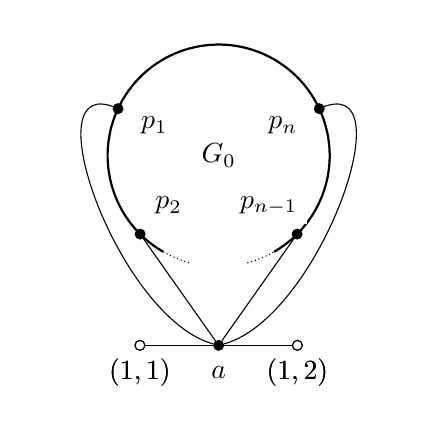
\begin{tikzpicture}[
  label distance=-5.5pt,
  thin,
  vertex/.style={circle,draw=black,fill=black,inner sep=1.25pt,
    minimum size =0mm},
  attach/.style={circle,draw=black,fill=white,inner sep=1.25pt,
    minimum size =0mm},
  dots/.style={circle,fill=black,inner sep=.5pt,
    minimum size= 0pt}]

% Path and Labels    
  \draw (-1,-2.41) -- (1,-2.41);
  
  \foreach \x /\n in {-1/ 1, 1/2}{
    \node at (\x,-2.41) [attach] {};
    \node at (\x,-2.75) {$(1,\n)$};
  }
    
  \node (a) at (0,-2.41) [vertex] {};
  \node at (0,-2.75) {$a$};
  
  \foreach \x /\n in {-1/ 1, 1/2}{
    \node at (\x,-2.41) [attach] {};
    \node at (\x,-2.75) {$(1,\n)$};
  }
  
% Graph  
  \draw[thick] (240:1.41) arc (240:-60:1.41);
  \draw[densely dotted] (240:1.41)  arc (240:255:1.41);
  \draw[densely dotted] (285:1.41)  arc (285:300:1.41);
  
  \foreach \i / \n /\t in {25 / n/ 15, 155 / 1/ 165, 225/ 2 / 120, 315 / {n-1}/60}{
    \node at (\i : .9) [rectangle,fill=white] {$p_\n$};
    \node at (\i : 1.41) [vertex] {};
  }
  \node at (0,0) [rectangle,fill=white] {$G_0$};

% Attaching Edges
  \foreach \i /\t in {25/15, 155/165}{
    \draw (\i:1.41) to[out=\i,in=\t] (a);
  }
  
  \foreach \i \in in {225,315}{
    \draw (\i:1.41) to (a);
  }

\end{tikzpicture}
  \caption{A type 1 R/T gadget.  Vertices of $G_0$ that are not part of the periphery $P = \{p_1,\ldots,p_n\}$ are not shown.}
  \label{fig:reversal_orig}
\end{figure}

Along these lines, we will investigate the scattering behavior of graphs where $\widehat{G}$ is of the form found in \fig{reversal_orig}.  While we still have that $\widehat{G}$ is of the form described in \sec{general_graphs}, the graph $G$ with the semi-infinite paths is that of a infinite path, with the graph $G_0$ attached to the vertex $a$.  As such, the graph that will be of more interest is the graph $G_0$ consisting of those vertices other than those along the infinite path.   We will label those vertices $p_i\in V(G_0)$ connected to the vertex $a$ as \emph{periphery} vertices, and we will label the set of periphery vertices as $P$.  In the special case that $|P| = 1$, or that a single vertex of $G_0$ is connected to $a$, we will call the gadget a type 2 R/T gadget (see \fig{RT_path} for an example of a type 2 R/T gadget).

For a given R/T gadget $\widehat{G}$, those momenta for which perfect reflection occurs shall be collected in the \emph{reflection set} which shall be denoted $\mathcal{R}$.  Similarly, those momenta for which perfect transmission occurs shall be collected in the \emph{transmission set} which shall be label $\mathcal{T}$. Note that these two sets have empty intersection, and that there isn't any nice relationship between them.

Let us now examine the scattering eigenstates for the graph $\widehat{G}$.  For any scattering state $\ket{\scat_{1} (k)}$, by examining the eigenvalue equation at vertices $(1,1)$ and $(1,2)$ we see that the amplitude at vertex $a$ satisfies
\begin{equation}
  \langle{a}\ket{\scat_{1} (k)} = 1 + R(k) = T(k).
\end{equation}
Thus perfect reflection at momentum $k$ occurs if and only if $R(k)=-1$ and $\langle{a}\ket{\scat_{1} (k)}=0$, while perfect transmission occurs if and only if $T(k)=1$ and $\langle{a}\ket{\scat_{1} (k)}=1$. Using this fact, we now derive conditions on the graph $G_0$ that determine when perfect transmission and reflection occur.

For any type 1 R/T gadget, we have necessary and sufficient conditions for momentum $k$ to be in the reflection set: $G_0$ should have an eigenvector for which the sum of amplitudes on the periphery is nonzero.
\begin{lemma}
Let $\widehat{G}$ be a type 1 R/T gadget. A momentum $k\in (-\pi,0)$ is in the reflection set $\mathcal{R}$ if and only if $G_0$ has an eigenvector $\ket{\chi_k}$ with eigenvalue $2\cos(k)$ satisfying
\begin{equation}
  \sum_{i=1}^{n} \braket{p_i}{\chi_k} \neq 0. \label{eq:sum_condition}
\end{equation}
\label{lem:reflect_reqs}
\end{lemma}

\begin{proof}
Let us first suppose that $\widehat{G}$ has perfect reflection at momentum $k$, i.e., $R(k)=-1$ and $\langle{a}\ket{\scat_{1} (k)}=0$. As $\langle{(1,1)}\ket{\scat_1(k)} = e^{-ik} - e^{ik}\neq 0$ and $\langle{(1,2)}\ket{\scat_1(k)}=0$, to satisfy the eigenvalue equation at vertex $a$, we have
\begin{equation}
  \sum_{j=1}^{n} \langle{p_j}\ket{\scat_1(k)} = e^{ik} - e^{-ik} \neq 0.
\end{equation}
Further, since $G_0$ only connects to vertex $a$ and the amplitude at this vertex is zero, the restriction of $\ket{\scat_1(k)}$ to $G_0$ must be an eigenvector of $G_0$ with eigenvalue $2\cos(k)$. Hence the condition is necessary for perfect reflection. 
 
Next suppose that $G_0$ has an eigenvector $\ket{\chi_k}$ with eigenvalue $2\cos(k)$ satisfying \eq{sum_condition}, with the sum equal to some nonzero constant $c$. Define a scattering state $\ket{\psi_k}$ on the Hilbert space of the full graph $G$ with amplitudes
\begin{equation}
  \braket{v}{\psi_k} = \frac{e^{ik} - e^{-ik}}{c} \braket{v}{\chi_k}
\end{equation}
for all $v \in V(G_0)$, $\braket{a}{\psi_k}=0$, and 
\begin{equation}
 \braket{(x,j)}{\psi_k}=\begin{cases} e^{-ikx}-e^{ikx} & j=1\\
0 & j=2
\end{cases}
\end{equation}
for all $x \in \posint$.

We claim that $\ket{\psi_k}$ is an eigenvector of $G$ with eigenvalue $2 \cos(k)$.  The state clearly satisfies the eigenvalue equation on the semi-infinite paths since it is a linear combination of states with momentum $\pm k$.  At vertices of $G_0$, the state is proportional to an eigenvector of $G_0$, and since the state has no amplitude at $a$, the eigenvalue equation is also satisfied at these vertices.  It remains to see that the eigenvalue equation is satisfied at $a$, but this follows immediately by a simple calculation.

Since $\ket{\psi_k}$ has the form of a scattering state with perfect reflection, we see that $R(k)=-1$ and $T(k)=0$ as claimed.
\end{proof}

In a similar manner, the following lemma gives a sufficient condition for a momentum $k$ to be in the transmission set (which is also necessary for type 2 gadgets).  Let $g_0$ denote the induced subgraph on $V(G_0)\setminus P$ where $P = \{p_i\colon i\in [n]\}$ is the periphery.

\begin{lemma}\label{lem:transmit_reqs}
Let $\widehat{G}$ be a type 1 R/T gadget and let $k\in (-\pi,0)$. Suppose $\ket{\xi_k}$ is an eigenvector of $g_0$ with eigenvalue $2\cos{k}$ and with the additional property that, for all $i \in [n]$,
\begin{equation}
\label{eq:trans_cond}
  \sum_{\substack{v \in V(g_0): \\ (v,p_i)\in E(G_0)}} \braket{v}{\xi_k} = c \neq 0 
\end{equation}
for some constant $c$ that does not depend on $i$. Then $k$ is in the transmission set $\mathcal{T}$. If $\hat{G}$ is a type 2 R/T gadget, then this condition is also necessary.
\end{lemma}

\begin{proof}
If $g_0$ has a suitable eigenvector $\ket{\xi_k}$ satisfying \eq{trans_cond}, define a scattering state $\ket{\psi_k}$ on the full graph $G$, with amplitudes $\langle a\ket{\psi_k}=1$, 
\begin{equation}
  \braket{v}{\psi_k} 
  = \begin{cases} -\frac{1}{c} \braket{v}{\xi_k} & v\in V(g_0)\\
  	0 & v \in P
\end{cases}
\label{eq:psik_c}
\end{equation}
in the graph $G_0$, and 
\begin{equation}
 \langle{(x,j)} \ket{\psi_k}=\begin{cases} e^{-ikx} & j=1\\
 e^{ikx} & j=2
\end{cases}
\end{equation}
for $x \in \posint$.  As in the proof of \lem{reflect_reqs}, the state $\ket{\psi_k}$ is clearly satisfies the eigenvalue equation (with eigenvalue $2\cos(k)$) at vertices on the semi-infinite paths and vertices of $g_0$.  The factor of $-\frac{1}{c}$ in \eq{psik_c} is chosen so that the eigenvalue condition is satisfied at vertices in $P$.  It is easy to see that the eigenvalue condition is also satisfied at $a$.

Since $\ket{\psi_k}$ is a scattering eigenvector of $G$ with eigenvalue $2\cos(k)$ and perfect transmission, we have $T(k)=1$.

Now suppose $\widehat{G}$ is a type 2 R/T gadget, with $P = \{p\}$.  Perfect transmission along with the eigenvalue equation at vertex $a$ implies
\begin{equation}
\braket{p}{\scat_1(k)} = 0,
\end{equation}
so the restriction of $\ket{\scat_1(k)}$ to $g_0$ must be an eigenvector (since $p$ is the only vertex connected to $g_0$).  The eigenvalue equation at $p$ gives
\begin{equation}
  \braket{a}{\scat_1(k)} 
  + \sum_{w \colon (w,p)\in E(G_0)} \braket{w}{\scat_1(k)} = 0 
  \quad\implies\quad
  \sum_{w \colon (w,p)\in E(G_0)} \braket{w}{\scat_1(k)} = -1.
\end{equation}
Hence the restriction of $\ket{\scat_1(k)}$ to $V(g_0)$ is an eigenvector of the induced subgraph, with the additional property that the sum of the amplitudes at vertices connected to $p$ is nonzero.
\end{proof}

With these two lemmas, if we can guarantee the form of the eigenstates for the graph $G_0$, we can guarantee certain momenta to be in either the reflection or the transmission set.


%%%%%%%%%%
\subsubsection{Explicit constructions}\label{sec:rt_ex}

While the two lemmas do give a nice abstract explanation for the construction of R/T gadgets, it doesn't provide us with a concrete example. As such, let us look at two simple graphs and examine when they satisfy the conditions of the lemmas.

As a first example, suppose $G_0$ is a finite path of length $l_1+l_2-2$ connected to $a$ at the $l_1$th vertex, as shown in \fig{RT_path}.  As this is a type 2 R/T gadget, we can then determine the reflection and transmission sets as a function of $l_1$ and $l_2$.


%%%%%%%%%
\begin{figure}
  \centering
  \tikzsetnextfilename{GS_RT_path}
  \begin{tikzpicture}[
  thin,
  vertex/.style={circle,draw=black,fill=black,inner sep=1.25pt,
    minimum size =0mm},
  attach/.style={circle,draw=black,fill=white,inner sep=1.25pt,
    minimum size =0mm},
  dots/.style={circle,fill=black,inner sep=.5pt,
    minimum size= 0pt}]
    
    \draw (-1,-1) -- (1,-1);
    \draw (0,0) -- (0,-1);
    
    \node[attach,label=270:{$(1,1)$}] at (-1,-1) {};
    \node[attach,label=270:{$(1,2)$}] at (1,-1) {};
    \node[vertex,label={[label distance=.25*\baselineskip]270:{$ a $}},] at (0,-1) {};
    \node[vertex] at (0,0) {};
    
    % left branch
    \draw (0,0) -- (135:1.5);
    \draw[densely dotted] (135:1.5) -- (135: 2.25);
    
    \draw[densely dotted] (135:2.75) -- (135:3.5);
    \draw (135:3.5) -- (135:5);
    
    \foreach \r in {1,5,4}{
      \node[vertex] at (135:\r) {};
    }
    

    \foreach \n /\p in {1/5,2/4,{l_1-1}/1}{
      \node at (135:\p) [label={225:$\n$}] {};
    }
    
    
    % right branch
    \draw (0,0) -- (45:1.5);
    \draw[densely dotted] (45:1.5) -- (45: 2.25);
    
    \draw[densely dotted] (45:3.75) -- (45:4.5);
    \draw (45:4.5) -- (45:6);
        
    \foreach \r in {1,6,5}{
      \node[vertex] at (45:\r) {};
    }    
    
    
    \foreach \n /\p in {{l_1}/0,{l_1+1}/1,{l_1+l_2-2}/5,{l_1+l_2-1}/6}{
      \node at (45:\p)[label=315:{$\n$}]{};
    }    

\end{tikzpicture}
  \caption{An R/T gadget built from a path of length $l_1+l_2-2$. }
  \label{fig:RT_path}
\end{figure}


Using \lem{reflect_reqs}, we see that perfect reflection occurs at momentum $k\in (-\pi,0)$ if and only if the path has an eigenvector with eigenvalue $2\cos(k)$ with non-zero amplitude on vertex $l_1$.  Recall that the path of length $L$ (where the length of a path is its number of edges) has eigenvectors $|\psi_j\rangle$ for $j\in [L+1]$ given by
\begin{equation}
  \langle x | \psi_j \rangle = \sin\left(\frac{ \pi j x}{L+2}\right)\label{eq:vecs_line}
\end{equation}
with eigenvalues $\lambda_j = 2 \cos(\pi j/(L+2))$.  Hence
\begin{equation}
  \mathcal{R}_{\mathrm{path}} = \left\{ -\frac{\pi j}{l_1 + l_2} \colon j\in [l_1 + l_2 - 1] \text{ and } \frac{jl_1}{l_1+l_2} \not\in \ZZ\right\}.
\end{equation}

To characterize the momenta at which perfect transmission occurs, consider the induced subgraph obtained by removing the $l_1$th vertex from the path of length $l_1+l_2-2$ (a path of length $l_1-2$ and a path of length $l_2-2$). We can choose bases for the eigenspaces of this induced subgraph so that each eigenvector has all of its support on one of the two paths, and has nonzero amplitude on only one of the vertices $l_1-1$ or $l_1+1$. Thus \lem{transmit_reqs} implies that $\widehat{G}$ perfectly transmits for all momenta in the set
\begin{equation}
  \mathcal{T}_{\mathrm{path}} = \left\{- \frac{\pi j}{l_1} \colon j\in [l_1-1]\right\} \cup \left\{-\frac{\pi j}{l_2 } \colon j \in [l_2-1]\right\}.
\end{equation}

As an explicit example, if we set $l_1 = l_2 = 2$, we get $\mathcal{T}_{\mathrm{path}} = \{-\frac{\pi}{2}\}$ and $\mathcal{R}_{\mathrm{path}} = \{-\frac{\pi}{4}, -\frac{3\pi}{4}\}$.


Now let us suppose $G_0$ is a cycle of length $r$. Labeling the vertices by $x \in [r]$, where $x=r$ is the vertex attached to the path (as shown in \fig{RT_cycle}), the eigenvectors of the $r$-cycle are
\begin{equation}
  \langle x | \phi_m\rangle = e^{{2 \pi i x m}/{r}}
\end{equation}
with eigenvalue $2 \cos(2 \pi m/r)$, where $m\in [r]$. For each momentum $k=-2 \pi m/r \in (-\pi,0)$, there is an eigenvector with nonzero amplitude on the vertex $r$ (i.e., $\langle r | \phi_m\rangle\neq 0$), so \lem{reflect_reqs} implies that perfect reflection occurs at each momentum in the set
\begin{equation}
  \mathcal{R}_{\mathrm{cycle}} = \left\{ -\frac{\pi j}{r} \colon \text{$j$ is even and $j\in [r-1]$}\right\}.
\end{equation}


%%%%%%%%%
\begin{figure}
  \centering
  \tikzsetnextfilename{GS_RT_cycle}
  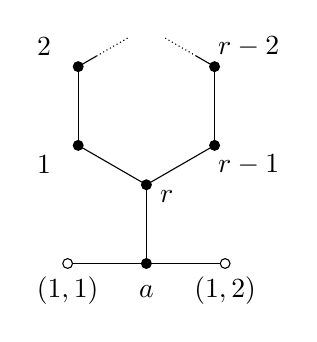
\begin{tikzpicture}[
  thin,
  vertex/.style={circle,draw=black,fill=black,inner sep=1.25pt,
    minimum size =0mm},
  attach/.style={circle,draw=black,fill=white,inner sep=1.25pt,
    minimum size =0mm},
  dots/.style={circle,fill=black,inner sep=.5pt,
    minimum size= 0pt}]
    \draw (-1,-2) -- (1,-2);
    \draw (0,-2) -- (0,-1);
    
    \node[attach] at (-1,-2) {};
    \node at (-1,-2.35) {$(1,1)$};
    \node[attach] at (1,-2) {};
    \node at (1,-2.35) {$(1,2)$};
    \node[vertex] at (0,-2) {};
    \node at (0,-2.35) {$a$};
    
    \foreach \t in {150, 210, 270, 330, 30}{
      \node[vertex] at (\t: 1) {};
    }
    
    \foreach \t in {210, 270, 330, 30}{
      \draw (\t:1) -- (\t - 60:1);
    }
    
    \draw (150:1) -- (135:.897);
    \draw (30:1) -- (45:.897);
    
    \draw[densely dotted] (45:.897) -- (75:.897);
    \draw[densely dotted] (135:.897) -- (105:.897);
    
    \foreach \t / \n in {210 / 1, 150 / 2, 30 / {r-2}, -30 / {r-1}}{
      \node at (\t:1.5) {$\n$};
    }
    
    \node at (.26,-1.15) {$r$};
  
\end{tikzpicture}
  \caption{An R/T gadget built from an $r$-cycle.}
  \label{fig:RT_cycle}
\end{figure}


To see which momenta perfectly transmit, we use \lem{transmit_reqs}. Consider the induced subgraph obtained by removing vertex $r$. This subgraph is a path of length $r-2$ and has eigenvalues $2\cos(\pi m/r)$ for $m \in [r-1]$ as discussed in the previous section. Using the expression \eq{vecs_line} for the eigenvectors, we see that the sum of the amplitudes on the two ends is nonzero for odd values of $m$.  Perfect transmission occurs for each of the corresponding momenta:  
\begin{equation}
  \mathcal{T}_{\mathrm{cycle}} = \left\{ -\frac{\pi j}{r} \colon \text{$j$ is odd and $j\in [r-1]$}\right\}.
\end{equation}

For example, the $4$-cycle (i.e., square) has $\mathcal{T}_{\mathrm{cycle}} = \{-\frac{\pi}{4},-\frac{3\pi}{4}\}$ and $\mathcal{R}_{\mathrm{cycle}} = \{-\frac{\pi}{2}\}$.  

%%%%%%%%%%%%%%%%%%%%%%%%%%%%%%%%%%%%%%
\subsubsection{Reversing reflection and transmission sets}\label{sec:reversal}

With these explicit examples of R/T gadgets, it will be useful to know how to interchange the reflection and transmission set.  Namely, if we have one gadget that transmits all momenta in $\mathcal{T}$ and reflects all momenta in $\mathcal{R}$, it will be useful to also have a gadget that reflects all momenta in $\mathcal{T}$ and transmits all momenta in $\mathcal{R}$.  Basically, we will be able to use these two gadgets together to construct gadgets with more interesting scattering behavior.

In particular, let $\widehat{G}$ be a type 2 R/T gadget, as seen in \fig{reversalRT}, and assume that it has a reflection set $\mathcal{R}$ and a transmission set $\mathcal{T}$.  We will construct a type 1 R/T gadget $\widehat{G}^{\leftrightarrow}$ with reflection set $\mathcal{R'} \supset \mathcal{T}$ and transmission set $\mathcal{T}' \supset \mathcal{R}$.  The graph $\widehat{G}^{\leftrightarrow}$ is depicted pictorially in \fig{reversal_changed}.

Explicitly, the R/T gadget $\widehat{G}^\leftrightarrow$ is obtained by taking two copies of the subgraph $g_0$ from the type 2 R/T gadget in \fig{reversalRT}, connecting both to a single additional vertex $u$, and connecting one copy of $g_0$ to the infinite path at $a$.  More concretely, for each vertex $w_j\in V(g_0)$, the graph $\widehat{G}^{\leftrightarrow}$ has two vertices $w_j^{(1)}$ and $w_j^{(2)}$, and the graph $\widehat{G}^\leftrightarrow$ inherits the edge set of $g_0$.  Additionally, for each $w_j\in V(g_0)$ connected to the periphery vertex $p$, we have that $w_j^{(i)}$ is connected to $u$, and $w_j^{(1)}$ is connected to $a$.

%%%%%%%%%%
\begin{figure}
  \centering
  \subfloat[][]{ 
    \tikzsetnextfilename{GS_reversalRT}
    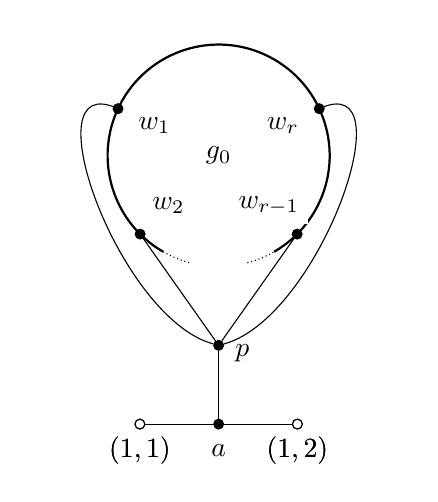
\begin{tikzpicture}[
  label distance=-5.5pt,
  thin,
  vertex/.style={circle,draw=black,fill=black,inner sep=1.25pt,
    minimum size =0mm},
  attach/.style={circle,draw=black,fill=white,inner sep=1.25pt,
    minimum size =0mm},
  dots/.style={circle,fill=black,inner sep=.5pt,
    minimum size= 0pt}]

% Path and Labels    
  \draw (-1,-3.41) -- (1,-3.41);
  
  \foreach \x /\n in {-1/ 1, 1/2}{
    \node at (\x,-3.41) [attach] {};
    \node at (\x,-3.75) {$(1,\n)$};
  }
    
  \node (a) at (0,-3.41) [vertex] {};
  \node at (0,-3.75) {$a$};
  
  \foreach \x /\n in {-1/ 1, 1/2}{
    \node at (\x,-3.41) [attach] {};
    \node at (\x,-3.75) {$(1,\n)$};
  }
  
  \node (v) at (0,-2.41) [vertex]{};
  \node at (0.3,-2.51) {$p$};
  \draw (v) to (a);
  
% Graph  
  \draw[thick] (240:1.41) arc (240:-60:1.41);
  \draw[densely dotted] (240:1.41)  arc (240:255:1.41);
  \draw[densely dotted] (285:1.41)  arc (285:300:1.41);
  
  \foreach \i / \n /\t in {25 / r/ 15, 155 / 1/ 165, 225/ 2 / 120, 315 / {r-1}/60}{
    \node at (\i : .9) [rectangle,fill=white] {$w_\n$};
    \node at (\i : 1.41) [vertex] {};
  }
  \node at (0,0) [rectangle,fill=white] {$g_0$};

% Attaching Edges
  \foreach \i /\t in {25/15, 155/165}{
    \draw (\i:1.41) to[out=\i,in=\t] (v);
  }
  
  \foreach \i \in in {225,315}{
    \draw (\i:1.41) to (v);
  }

\end{tikzpicture}
    \label{fig:reversalRT}
  }
  \qquad
  \subfloat[][]{
    \tikzsetnextfilename{GS_reversal_changed}
    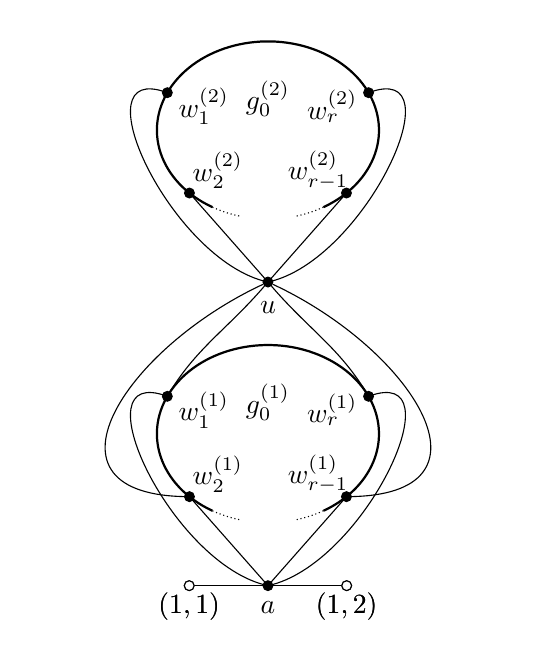
\begin{tikzpicture}[
  yscale = 0.8,
  label distance=-5.5pt,
  thin,
  vertex/.style={circle,draw=black,fill=black,inner sep=1.25pt,
    minimum size =0mm},
  attach/.style={circle,draw=black,fill=white,inner sep=1.25pt,
    minimum size =0mm},
  dots/.style={circle,fill=black,inner sep=.5pt,
    minimum size= 0pt}]

% Path and Labels    
  \draw (-1,-2.41) -- (1,-2.41);
  
  \foreach \x /\n in {-1/ 1, 1/2}{
    \node at (\x,-2.41) [attach] {};
    \node at (\x,-2.75) {$(1,\n)$};
  }
    
  \node (a) at (0,-2.41) [vertex] {};
  \node at (0,-2.75) {$a$};
  
  \foreach \x /\n in {-1/ 1, 1/2}{
    \node at (\x,-2.41) [attach] {};
    \node at (\x,-2.75) {$(1,\n)$};
  }
  
  \node (v) at (0,2.41) [vertex] {};
  \node at (0,2) {$u$};
  
% Graphs (both)

\foreach \j/\of in {1/0,2/4.82}{
\begin{scope}[yshift=\of cm]
  \foreach \i / \n /\t in {25 / r/ 15, 155 / 1/ 165, 225/ 2 / 120, 315 / {r-1}/60}{
    \node at (\i : .9) [rectangle,fill=white] {$w_\n^{(\j)}$};
    \node at (\i : 1.41) [vertex] {};
  }
  \node at (0,0.5) [rectangle,fill=white] {$g_0^{(\j)}$};
  
  \draw[thick] (240:1.41) arc (240:-60:1.41);
  \draw[densely dotted] (240:1.41)  arc (240:255:1.41);
  \draw[densely dotted] (285:1.41)  arc (285:300:1.41);

% Attaching Edges
  \foreach \i /\t in {25/15, 155/165}{
    \draw (\i:1.41) to[out=\i,in=\t] (0,-2.41);
  }
  
  \foreach \i \in in {225,315}{
    \draw (\i:1.41) to (0,-2.41);
  }
  
\end{scope}
}

  \draw (25:1.41) to [out = 115,in=-55] (v);
  \draw (155:1.41) to [out=65,in=-125] (v);
  \draw[looseness=1.5] (225:1.41) to[out=180,in=210] (v);
  \draw[looseness=1.5] (315:1.41) to[out=0,in=-30] (v);
\end{tikzpicture}
    \label{fig:reversal_changed}
   }
   \caption{\subfig{reversalRT}  A type 2 R/T gadget, (i.e., a type 1 gadget with $|P| = 1$).  \subfig{reversal_changed}  The R/T gadget $\widehat{G}^\leftrightarrow$ reversing the reflection and transmission sets of \subfig{reversalRT}.}
   \label{fig:reversal}
\end{figure}

With this definition, we now prove that the graph $\widehat{G}^\leftrightarrow$ reverses the reflection and transmission sets of $\widehat{G}$.

\begin{lemma}\label{lem:reversal_graph}
Let $\widehat{G}$ be a type 2 R/T gadget with transmission set $\mathcal{T}$ and reflection set $\mathcal{R}$.  The type 1 R/T gadget $\widehat{G}^{\leftrightarrow}$ defined above has transmission set $\mathcal{T}' \supseteq \mathcal{R}$ and reflection set $\mathcal{R}' \supseteq \mathcal{T}$.
\end{lemma}
\begin{proof}
First consider a momentum $k\in \mathcal{T}$. Using the condition derived in \lem{transmit_reqs}, we see that $g_0$ has an eigenvector $\ket{\xi_k}$ with eigenvalue $2\cos(k)$ where the sum of the amplitudes on vertices $w_1,\ldots,w_r$ is nonzero.  Now consider the induced subgraph $G_{0}^{\leftrightarrow}$ of \fig{reversal_changed} obtained by removing vertices $(1,1)$, $(1,2)$, and $a$. This subgraph has an eigenvector $|\chi^{\leftrightarrow}_k\rangle$ with eigenvalue $2\cos(k)$ given by
\begin{equation}
  \langle v^{(i)} \ket{\chi^{\leftrightarrow}_k}= (-1)^i \langle v\ket{\xi_k} \quad \text{ and } \quad \langle{u}\ket{\chi^{\leftrightarrow}_k} = 0
\end{equation}
for all vertices $v\in V(g_0)$ and for $i \in \{1,2\}$.  The fact that $\ket{\chi_k^{\leftrightarrow}}$ is an eigenvector follows from the fact that $\ket{\xi_k}$ is an eigenvector of $g_0$.  Additionally, we have that
\begin{equation}
  \sum_{j=1}^{r} \langle{w^{(1)}_j} \ket{\chi^{\leftrightarrow}_k} = - \sum_{j=1}^{r} \langle{w_j} \ket{\xi_k} \neq 0.
\end{equation}
Using \lem{reflect_reqs}, we see that perfect reflection occurs at momentum $k$, and thus $\mathcal{T} \subseteq \mathcal{R}'$.

Next suppose $k\in \mathcal{R}$. \lem{reflect_reqs} states that $G_0$ has an eigenvector $|\chi_k\rangle$ with eigenvalue $2\cos(k)$ such that $\langle p \ket{\chi_k} \neq 0$.  Now consider the induced subgraph $g_0^{\leftrightarrow}$ of \fig{reversal_changed} obtained by removing vertices $(1,1)$, $(1,2)$, $a$, and $w^{(1)}_1,\ldots,w^{(1)}_{r}$. This graph has an eigenvector $\ket{\xi^{\leftrightarrow}_k}$ with eigenvalue $2\cos(k)$ defined by
\begin{equation}
  \langle v \ket{\xi^{\leftrightarrow}_k} = \begin{cases} \langle{v}\ket{\chi_k}& \text{for }v\in V(g_0^{(2)}) \\
    \langle{p}\ket{\chi_k} & v = u\\
0 &\text{otherwise.} \end{cases}
\end{equation}
To see that this is an eigenvector, observe that $g_0^{\leftrightarrow}$ is a disconnected graph and $\ket{\chi_k}$ is an eigenvector of one of its components.  Using this and \lem{transmit_reqs} (since $u$ is the only vertex adjacent to the periphery of $\hat{G}^{\leftrightarrow}$ with non-zero amplitude), we see that $k\in \mathcal{T}'$, so $\mathcal{R} \subseteq \mathcal{T}'$.
\end{proof}


%%%%%%%%%%%%%%%%%%%%%%%%%%%%%%%%%%%%%%%%%%%%%%%%%%%%%%%%%%%%%%%%%

\subsection{Momentum switches}

To construct a momentum switch between a given pair of momenta, it will be worthwhile to first construct two R/T gadgets between the momenta, with the two gadgets having swapped reflection and transmission sets.  We can then construct something like a railroad switch, by placing the two gadgets immediately after a 3-claw.  With this design, the incident wavepacket will only see one of the two outgoing paths, and the resulting $S$-matrix will be exactly what we want.

In particular, we can construct a momentum switch between the reflection and transmission sets $\mathcal{R}$ and $\mathcal{T}$ of a type 2 R/T gadget.  We attach the gadget and its reversal (defined in \sec{reversal}) to the leaves of a claw, as shown in \fig{gen_mom_con}.  Specifically, given a type 2 R/T gadget $\widehat{G}$, the corresponding momentum switch $\widehat{G}^{\prec}$ consists of a copy of $G_0$, a copy of $G_{0}^{\leftrightarrow}$, and a claw, with the three leaves of the claw acting as the terminal vertices.  Vertex $p$ of $G_0$ is connected to leaf $2$ of the claw, and vertices $w_1^{(1)},\ldots,w_r^{(1)}$ of $G_{0}^{\leftrightarrow}$ are each connected to leaf $3$ of the claw.

Intuitively, the momentum switch acts the same as a railroad switch.  For momenta in the transmission set, the gadget perfectly transmits while its reversal perfectly reflects, so the claw is effectively a path connecting terminals 1 and 2.  For momenta in the reflection set, the roles of transmission and reflection are reversed, so the claw is effectively a path connecting terminals 1 and 3.

%%%%%%%%%%%%%%%%
\begin{figure}
  \centering
  \tikzsetnextfilename{GS_gen_mom_con}
  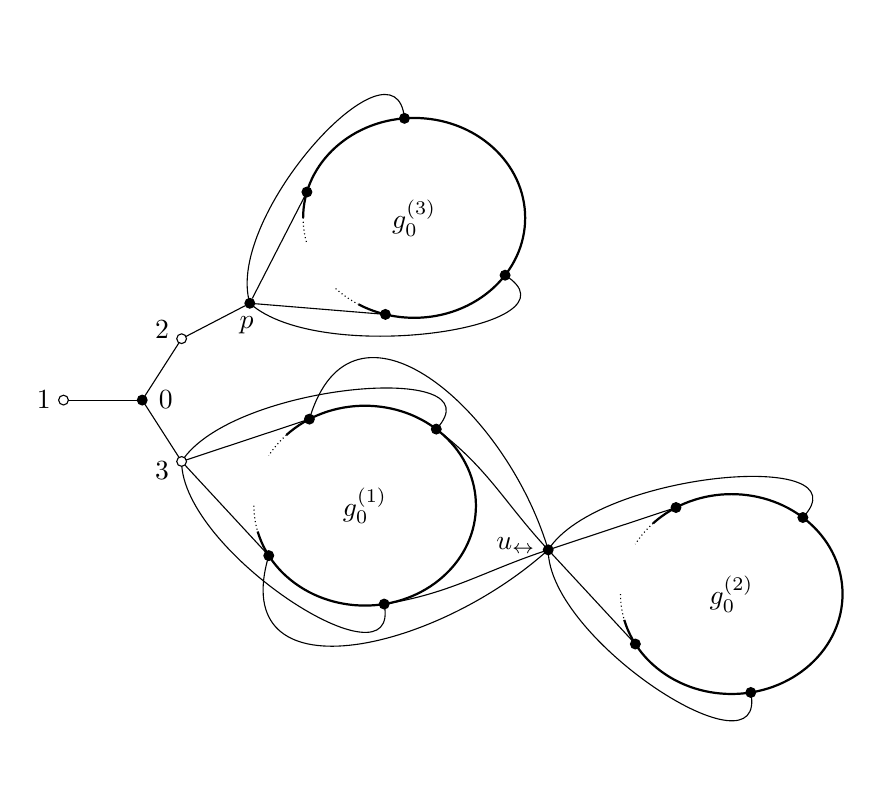
\begin{tikzpicture}[
  yscale = .9,
  label distance=-5.5pt,
  thin,
  vertex/.style={circle,draw=black,fill=black,inner sep=1.25pt,
    minimum size =0mm},
  attach/.style={circle,draw=black,fill=white,inner sep=1.25pt,
    minimum size =0mm},
  dots/.style={circle,fill=black,inner sep=.5pt,
    minimum size= 0pt}]

%%%%%%%%%%%%%%
% G^RT_\leftrightarrow graph
\begin{scope}[yshift=-.866 cm,xshift=.5cm,rotate=255,yshift = 2.41cm]

% Path and Labels    
  
  \node (v) at (0,2.41) [vertex] {};
  \node at (.05,2) {$u_\leftrightarrow$};
  
% Graphs

\foreach \j/\of in {1/0,2/4.82}{
\begin{scope}[yshift=\of cm]
  \foreach \i / \n /\t in {25 / n/ 15, 155 / 1/ 165, 225/ 2 / 120, 315 / {n-1}/60}{

    \node at (\i : 1.41) [vertex] {};
  }
  \node at (0,0) [rectangle,fill=white] {$g_0^{(\j)}$};
  
  \draw[thick] (240:1.41) arc (240:-60:1.41);
  \draw[densely dotted] (240:1.41)  arc (240:255:1.41);
  \draw[densely dotted] (285:1.41)  arc (285:300:1.41);
  
% Attaching Edges
  \foreach \i /\t in {25/15, 155/165}{
    \draw (\i:1.41) to[out=\i,in=\t] (0,-2.41);
  }
  
  \foreach \i \in in {225,315}{
    \draw (\i:1.41) to (0,-2.41);
  }
  
\end{scope}
}

  \draw (25:1.41) to [out = 115,in=-55] (0,2.41);
  \draw (155:1.41) to [out=65,in=-125] (0,2.41);
  \draw[looseness=1.5] (225:1.41) to [out=180,in=210] (0,2.41);
  \draw[looseness=1.5] (315:1.41) to [out=0,in=-30] (0,2.41);

\end{scope}

%%%%%%%%%%%%%%%%%%%%%%%%
% G^RT graph
\begin{scope}[xshift = .5 cm, yshift = .866 cm, rotate = -60, yshift = 3.41 cm]
% Path and Labels    
  
  \node (v) at (0,-2.41) [vertex]{};
  \node at (0.25,-2.6) {$p$};
  \draw (v) -- (0,-3.41); 
  
% Graph  
  \foreach \i / \n /\t in {25 / n/ 15, 155 / 1/ 165, 225/ 2 / 120, 315 / {n-1}/60}{

    \node at (\i : 1.41) [vertex] {};
  }
  \node at (0,0) [rectangle,fill=white] {$g_0^{(3)}$};
  
  \draw[thick] (240:1.41) arc (240:-60:1.41);
  \draw[densely dotted] (240:1.41)  arc (240:255:1.41);
  \draw[densely dotted] (285:1.41)  arc (285:300:1.41);

% Attaching Edges
  \foreach \i /\t in {25/15, 155/165}{
    \draw (\i:1.41) to [out=\i,in=\t] (0,-2.41);
  }
  
  \foreach \i \in in {225,315}{
    \draw (\i:1.41) to (v);
  }
  
\end{scope}

%%%%%%%
% Center stuff
\foreach \t in {60, 180, 300}{
  \draw (0,0) -- (\t:1);
}

\node (0) at (0,0) [vertex] {};
\node (1) at (180:1) [attach] {};
\node (2) at (60:1) [attach]{};
\node (3) at (-60:1) [attach]{};

\node at (0:.3) {$0$};
\node at (-1.25,0) {$1$};
\node at (.25,1) {$2$};
\node at (.25,-1) {$3$};
\end{tikzpicture}
  \caption{A momentum switch $\hat G^\prec$ built from a type 2 R/T gadget and its reversal.}
  \label{fig:gen_mom_con}
\end{figure}

We can now prove that this gadget acts as a momentum switch, by constructing the desired scattering eigenstates.

\begin{lemma}\label{lem:mom_switch_construction}
Let $\widehat{G}$ be a type 2 R/T gadget with reflection set $\mathcal{R}$ and transmission set $\mathcal{T}$.  The gadget $\hat{G}^{\prec}$ described above is a momentum switch between the sets $\mathcal{R}$ and $\mathcal{T}$.
\end{lemma}
\begin{proof}

We construct a scattering eigenstate for each momentum $k\in \mathcal{T}$ with perfect transmission from path 1 to path 2, and similarly construct a scattering eigenstate for each momentum $k^{\prime}\in \mathcal{R}$ with perfect transmission from 1 to 3.  These eigenstates show that $S_{2,1}(k) = 1$ and $S_{3,1}(k^\prime) = 1$. Since the S-matrix is symmetric and unitary, this gives the complete form of the S-matrix for all momenta in $\mathcal{R}\cup\mathcal{T}$.  In particular, this shows that $\hat{G}^{\prec}$ is a momentum switch between $\mathcal{R}$ and $\mathcal{T}$.

We first construct the scattering states for momenta $k\in \mathcal{T}$.  \lem{transmit_reqs} shows that the graph $g_0$ has a $2\cos(k)$-eigenvector $\ket{\xi_k}$ satisfying equation \eq{trans_cond} with some nonzero constant $c$. We define a state $\ket{\mu_k}$ on $G^{\prec}$ and we show that it is a scattering eigenstate with perfect transmission between paths $1$ and $2$.   The amplitudes of $\ket{\mu_k}$ on the semi-infinite paths and the claw are
\begin{equation}
  \langle (x,1)|\mu_k\rangle=e^{-ikx} \qquad 
  \langle 0|\mu_k\rangle=1 \qquad 
  \langle (x,2)|\mu_k\rangle=e^{ikx} \qquad
  \langle (x,3)|\mu_k\rangle=0.
\end{equation}
The rest of the graph consists of the three copies of the subgraph $g_0$ and the vertices $p$ and $u_{\leftrightarrow}$. The corresponding amplitudes are
\begin{equation}
  \braket{v}{\mu_k} =
  \begin{cases}
	  -\frac{1}{c}\braket{v}{\xi_k} & v\in V(g^{(1)}_0) \\
    \frac{1}{c}\braket{v}{\xi_k} & v \in V(g^{(2)}_0) \\
	  -\frac{e^{ik}}{c} \braket{v}{\xi_k} & v \in V(g^{(3)}_0) \\
  	0 & v=p \text{ or } v=u_{\leftrightarrow}.
  \end{cases}
\end{equation}

We claim that $\ket{\mu_k}$ is an eigenstate of the Hamiltonian with eigenvalue $2\cos(k)$.  As in previous proofs, the state clearly satisfies the eigenvalue condition on the semi-infinite paths and at the vertices of $G_0$ and $G_0^\leftrightarrow$, and the factors of $\frac{1}{c}$ in the above equation are chosen so that the state also satisfies the eigenvalue condition at vertices $p$ and $u_\leftrightarrow$. Since $\ket{\mu_k}$ is a scattering state with perfect transmission from path 1 to path 2, we see that $S_{2,1}(k) = 1$.

We now construct an eigenstate $\ket{\nu_{k^\prime}}$ with perfect transmission from path 1 to path 3 for each momentum $k^\prime \in \mathcal{R}$.  This state has the form
\begin{equation}
  \langle (x,1)|\nu_{k^\prime}\rangle=e^{-i k^\prime x} \qquad 
  \langle 0|\nu_{k^\prime}\rangle=1 \qquad 
  \langle (x,2)|\nu_{k^\prime}\rangle=0 \qquad
  \langle (x,3)|\nu_{k^\prime}\rangle=e^{i k^\prime x}
\end{equation}
on the semi-infinite paths and the claw.  \lem{reflect_reqs} shows that $G_0$ has a $2\cos(k^\prime)$-eigenstate $\ket{\chi_{k^\prime}}$ with $\braket{p}{\chi_{k'}} \ne 0$, which determines the form of $\ket{\nu_{k^\prime}}$ on the remaining vertices:
\begin{equation}
  \braket{v}{\nu_{k^\prime}} =
  \begin{cases}
	  -\frac{1}{\braket{p}{\chi_{k'}}} \braket{v}{\chi_{k^\prime}} & v \in V(G_0) \\
	  -\frac{e^{ik'}}{\braket{p}{\chi_{k'}}} \braket{v}{\chi_{k^\prime}} & v \in V(g_0^{(2)}) \\
	  -e^{ik'} & v=u^\leftrightarrow \\
    0 & \text{otherwise}.
  \end{cases} 
\end{equation}
As before, it is easy to check that this a momentum-$k^\prime$ scattering state with perfect transmission from path 1 to path 3, so $S_{3,1}(k^\prime)=1$.

Thus the gadget from \fig{gen_mom_con} is a momentum switch between $\mathcal{R}$ and $\mathcal{T}$.
\end{proof}

%%%%%%
\subsubsection{Explicit example}

Using this construction for momentum switches, we can obtain a momentum switch from any of the examples discussed in \sec{rt_ex}.  Explicitly, using the R/T gadget built from the 3-cycle, we get a momentum switch between $-\frac{\pi}{3}$ and $-\frac{2\pi}{3}$, as shown in \fig{mom_switch_ex}.  More generally, using an $r$-cycle, we obtain a switch between momenta of the form $-\frac{\pi j}{r}$ with odd or even values of $j$.  As another example, using a path of length $4$ connected at the center vertex, we obtain a switch between $-\frac{\pi}{4}$ and $-\frac{\pi}{2}$.

\begin{figure}
  \centering
  \tikzsetnextfilename{GS_mom_switch_ex}
  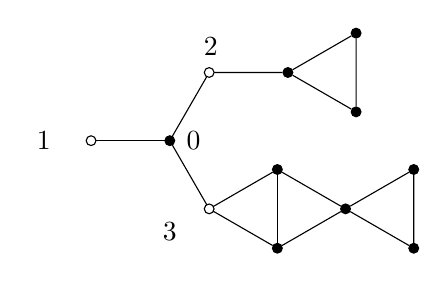
\begin{tikzpicture}[
  label distance=-5.5pt,
  thin,
  vertex/.style={circle,draw=black,fill=black,inner sep=1.25pt,
    minimum size =0mm},
  attach/.style={circle,draw=black,fill=white,inner sep=1.25pt,
    minimum size =0mm},
  dots/.style={circle,fill=black,inner sep=.5pt,
    minimum size= 0pt}]

\begin{scope}[yshift = .866cm, xshift = .5cm,rotate=0]

  \node (b) at (1,0) [vertex] {};
  \node (c) at (1.866,.5) [vertex] {};
  \node (d) at (1.866,-.5) [vertex] {};
  
  \draw (0,0) -- (b) -- (c) -- (d) -- (b);
\end{scope}

\begin{scope}[yshift = -.866cm, xshift = .5cm,rotate= -90]
  \node (e) at (.5,.866) [vertex] {};
  \node (f) at (-.5,.866) [vertex] {};
  \node (g) at (0,1.732) [vertex] {};
  \node (h) at (.5,2.598) [vertex] {};
  \node (i) at (-.5,2.598) [vertex]{};
  
  \draw (0,0) -- (e) -- (g) -- (h) -- (i) -- (g) -- (f) -- (0,0);
  \draw (e) -- (f);

\end{scope}

%%%%%%%
% Center stuff
\foreach \t in {60, 180, 300}{
  \draw (0,0) -- (\t:1);
}

\node (0) at (0,0) [vertex] {};
\node (1) at (180:1) [attach] {};
\node (2) at (60:1) [attach]{};
\node (3) at (-60:1) [attach]{};

\node at (0:.3) {$0$};
\node at (-1.6,0) {$1$};
\node at (0.52,1.2) {$2$};
\node at (0,-1.15) {$3$};

\end{tikzpicture}
  \caption{A momentum switch between $-\frac{\pi}{3}$ and $-\frac{2\pi}{3}$.}
  \label{fig:mom_switch_ex}
\end{figure}


%%%%%%%%%%%%%%%%%%%%%%%%%%%%%%%%%%%%%%
\subsection{Encoded unitaries}

While there is no known efficient method to find graphs that fixed scattering behavior, it is possible to search over all small graphs in order to find gadgets with some particular scattering behavior.  This was the manner in which the gadgets for most known scattering results were found, such as in Childs' original universality proof for graph scattering \cite{Chi09} and Childs, Gosset, and Webb's universality result \cite{MPQW}.  Additionally, Blumer, Underwood, and Feder have a paper \cite{BUF11} in which they searched over all graphs with up to 9 vertices for scattering behavior at particular momentum.

Essentially, the main idea behind this method is a brute force search.  Since we can easily compute the scattering matrix for a particular graph at a particular momentum, if we want to find a graph that has some prescribed scattering behavior, we simply assume that such a graph exists and search for it over all graphs, starting with those having a small number of vertices.  While this exhaustive search is not guaranteed to find such a graph, a surprising number of systems can be found with this structure.  In particular, if we restrict ourselves to momenta that are simple multiples of $\pi$, such as $-\frac{\pi}{2}$ or $-\frac{\pi}{4}$, then most simple scattering behaviors can be found.  

Of particular interest to us will be gadgets with four terminal vertices, such that the scattering matrix at some particular momenta takes the form
\begin{equation}
  S(k) = \begin{pmatrix} 0 & U^T\\
    U & 0\end{pmatrix}. \label{eq:encoded_scat}
\end{equation}
Namely, if we use a dual-rail encoding for a qubit, and think of one pair of semi-infinite paths as the input rails and the other pair as the output rails, then after scattering this gadget will have applied the unitary $U$ to the encoded qubit.

Later in the thesis, we will be interested in finding a universal gate set for both $-\frac{\pi}{4}$ and $-\frac{\pi}{2}$.  As such, we can take as examples those graphs that will be of interest to us later.   


%%%%%%%%%%%%%%%%%%%%%%%%%%%%
\begin{figure}
  \centering
  \subfloat[][]{ 
    \tikzsetnextfilename{GS_pi_4_phase}
    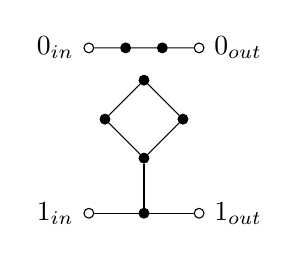
\begin{tikzpicture}
  [ scale=0.7,inner/.style={circle,draw=black!100,fill=black!100,inner sep = 1.25pt},
    attach/.style={circle,draw=black!100,fill=black!0,thin,inner sep = 1.25pt}]
  \node (0) at (-1,      0)      [attach,label=left:$1_\text{in}$] {};
  \node (1) at ( 0,      0)      [inner]  {};
  \node (2) at ( 1,      0)      [attach,label=right:$1_\text{out}$] {};  
  \node (3) at ( 0,      1)      [inner]  {};
  \node (4) at ( 0,      2.4142) [inner]  {};
  \node (5) at (-0.7071, 1.7071) [inner]  {};
  \node (6) at ( 0.7071, 1.7071) [inner]  {};
  \node (7) at (-1,      3)      [attach,label=left:$0_\text{in}$] {};
  \node (8) at (-0.3333, 3)      [inner]  {};
  \node (9) at ( 0.3333, 3)      [inner]  {};
  \node (10)at ( 1,      3)      [attach,label=right:$0_\text{out}$] {};

  \draw (1) to (0) [thin];
  \draw (1) to (2) [thin];
  \draw (1) to (3) [thin];
  \draw (3) to (5) [thin];
  \draw (3) to (6) [thin];
  \draw (5) to (4) [thin];
  \draw (6) to (4) [thin];  
  \draw (8) to (7) [thin];
  \draw (8) to (9) [thin];
  \draw (9) to (10)[thin];
\end{tikzpicture}
    \label{fig:pi_4_phase}
  }
  \qquad
  \subfloat[][]{
    \tikzsetnextfilename{GS_pi_4_basis_change}
    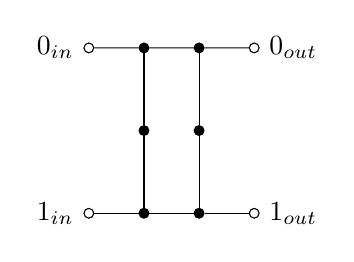
\begin{tikzpicture}
  [ scale=0.7,
    yscale=1.5,
    inner/.style={circle,draw=black!100,fill=black!100,inner sep = 1.25pt},
    attach/.style={circle,draw=black!100,fill=black!0,thin,inner sep = 1.25pt}]

  \node (1) at ( 0, 2) [inner]  {};
  \node (2) at ( 0, 0) [inner]  {};
  \node (3) at ( 1, 2) [inner]  {};
  \node (4) at ( 1, 0) [inner]  {};
  \node (5) at ( 0, 1) [inner]  {};
  \node (6) at ( 1, 1) [inner]  {};
  \node (7) at (-1, 2) [attach,label=left:$0_\text{in}$] {};
  \node (8) at (-1, 0) [attach,label=left:$1_\text{in}$] {};
  \node (9) at ( 2, 2) [attach,label=right:$0_{\text{out}}$] {};
  \node (0) at ( 2, 0) [attach,label=right:$1_{\text{out}}$] {};

  \draw (7) to (1) [thin];
  \draw (8) to (2) [thin];
  \draw (3) to (9) [thin];
  \draw (4) to (0) [thin];
  \draw (1) to (3) [thin];
  \draw (1) to (5) [thin];
  \draw (2) to (4) [thin];
  \draw (2) to (5) [thin];
  \draw (3) to (6) [thin];
  \draw (4) to (6) [thin];
\end{tikzpicture}
    \label{fig:pi_4_basis_change}
   }
   \caption{Encoded one-qubit gates at $k = -\frac{\pi}{4}$.  \subfig{pi_4_phase}  A phase gate.  \subfig{pi_4_basis_change}  Basis-changing gate.}
   \label{fig:reversal}
\end{figure}

%%%%%%%%%%%%%%%%%
\begin{figure}
  \centering
  \tikzsetnextfilename{GS_pi_2_had}
  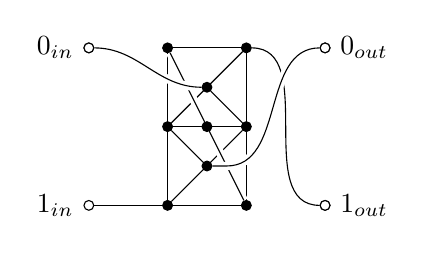
\begin{tikzpicture}
  [ scale=1,
    thin,
    attach/.style={circle,fill=white,draw=black,
      inner sep=1.25pt,minimum size=0pt},
    vert/.style={circle,draw=black,fill=black,
      inner sep=1.25pt,minimum size=0pt}]
  
    \node (0inhad) at (0,2) [attach]{};
    \node (1inhad) at (0,0) [attach]{};
    \node (0outhad) at (3,2) [attach]{};
    \node (1outhad) at (3,0) [attach]{};
    
    \node (1had) at (1,0) [vert]{};
    \node (2had) at (2,0) [vert]{};
    \node (3had) at (1.5,.5) [vert]{};
    \node (4had) at (1,1) [vert]{};
    \node (5had) at (1.5,1) [vert] {};
    \node (6had) at (2,1) [vert] {};
    \node (7had) at (1.5,1.5) [vert]{};
    \node (8had) at (1,2) [vert]{};
    \node (9had) at (2,2) [vert]{};

    \draw (8had) -- (1had);
    \draw (9had) -- (2had);
    \draw (4had) -- (9had);
    \draw (1had) -- (6had);
    \draw (4had) -- (6had);
    \draw (3had) -- (4had);
    \draw (7had) -- (6had);
    \draw (1inhad) -- (2had);
    \draw (8had) -- (9had);
    \draw (8had) -- (5had)[line width=3pt,white];
    \draw (5had) -- (2had)[line width=3pt,white];
    \draw (8had) -- (2had);
    
    \draw (9had) to[out=0,in=180] (1outhad) [looseness=.3];
    \draw (0inhad) to[out=0,in=180] (7had)[line width = 3pt,white];
    \draw (0inhad) to[out=0,in=180] (7had);

    \draw (3had) --(1.75,.5) to[out=0,in=180] (0outhad)[line width =3pt,white];
    \draw (3had) --(1.75,.5) to[out=0,in=180] (0outhad);

    \node at (0inhad) [attach]{};
    \node at (1outhad) [attach]{};
    \node at (0outhad) [attach]{};


  \node at (1inhad.west) [left] {$1_{\text{in}}$};
  \node at (0inhad.west) [left] {$0_{\text{in}}$};
  \node at (0outhad.east) [right] {$0_{\text{out}}$};
  \node at (1outhad.east) [right] {$1_{\text{out}}$};
\end{tikzpicture}
  \caption{Graph implementing a Hadamard gate at $k = -\frac{\pi}{2}$.
    \label{fig:pi_2_had}}
\end{figure}


In particular, we have that the graph in \fig{pi_4_phase} has a scattering matrix of the form of equation \eq{encoded_scat} at momentum $k= -\frac{\pi}{4}$, with 
\begin{equation}
  U = \begin{pmatrix}
    e^{- i \frac{\pi}{4}} & 0\\
    0 & 1 
  \end{pmatrix},
\end{equation}
while the gadget in \fig{pi_4_basis_change} also has a scattering matrix of the form \eq{encoded_scat} at momentum $k=-\frac{\pi}{4}$, where
\begin{equation}
  U = -\frac{i}{\sqrt{2}}\begin{pmatrix}
    1 & -i\\
    -i & 1 
  \end{pmatrix}.
\end{equation}

Similarly, we have that at $k = -\frac{\pi}{2}$, the graph of \fig{pi_2_had} has a scattering matrix of the form \eq{encoded_scat}, with
\begin{equation}
  U = -\frac{e^{i \frac{\pi}{4}}}{\sqrt{2}}\begin{pmatrix}
    1 & 1\\
    1 & -1 
  \end{pmatrix}.
\end{equation}

With these examples, we then have a universal gate set for single-qubit unitaries at $-\frac{\pi}{4}$, which will be sufficient for our eventual purposes.  


%%%%%%%%%%%%%%%%%%%%%%%%%%%%%%%%%%%%%%%%%%%%%%%%%%%%%%%%%%%%%%%%%

%%%%%%%%%%%%%%%%%%%%%%%%%%%%%%%%%%%%%%%%%%%%%%%%%%%%%%%%%%%%%%%%%
\section{Various facts about scattering}

While the previous constructions yield graphs with particular behavior which will be useful when attempting to construct scattering algorithms, we will also want to understand some simple relations between graphs and their respective scattering matrices.  In particular, understanding what properties are necessary in order to have a given scattering matrix, and understanding the relation between various the scattering matrices of various momenta will be useful in constructing additional scattering graphs.

\subsection{Degree-3 graphs are sufficient}

One of the most simple assumptions that could be made is that certain scattering behaviors require high degree graphs.  In particular, having many connections might allow for additional correlations between outputs on larger graphs.  

If we restrict our attention to a finite number of rational momenta, however, this does not turn out to be the case.  We can show that any graph can be replaced by a degree-three graph with a identical scattering behavior at some fixed momenta.  In particular, we will show that a single vertex can be replaced by a finite path while still satisfying the eigenvalue equation at the fixed momenta, where the length of the path is dependent on the fixed momenta.

As degree two graphs are the graph joins of cycles and paths, degree three graphs are the smallest graphs to have nontrivial scattering behaviors.  This lemma shows that, in a certain sense, they are also all that are required.

\begin{lemma} Let $\widehat{G}$ be a finite graph, and let $M$ be a finite set of rational multiples of $\pi$.  If $v\in V(G)$ is a degree $d$ vertex, there exists a graph $H$ that extends $G$ with the vertex $v$ being replaced by a degree-$(\lceil \frac{d}{2}\rceil +1)$ subgraph such that the scattering matrices at the momenta $k\in M$ are preserved.
\label{lem:degree_reduction}
\end{lemma}
\begin{proof}
  The main idea behind this proof is to partition the vertices adjacent to $v$ into two sets, and then replace $v$ by a finite path, with the two sets connected to opposites ends of the finite path.  By choosing the length of the path correctly, we can show that the amplitudes at either end of the path are the same as the amplitude on $v$ at each momenta in $M$, and thus the eigenvalue equation remains satisfied without changing the scattering behavior.  
  
  In particular, let $v$ be the degree $d$ vertex in $G$, and let $S = \{w\in V(G) : w\sim v\}$ be the set of vertices adjacent to $v$.  Additionally, let us arbitrarily partition $S$ into two sets, $S_1$ and $S_2$, such that $\big||S_1|-|S_2|\big| \leq 1$.
  
  As each $k\in M$ is a rational multiple of $\pi$, there exists some $m\in \NN^+$ such that $\frac{mk}{2\pi} \in \NN$ for all $k\in M$.  Let us then examine the graph $H$ where $v$ is replaced by a path of length $m$, and where $S_1$ is attached to one end of the path while $S_2$ is attached to the other end.  Explicitly:
  \begin{align}
    V(H) &= \big(V(G)\setminus \{v\}\big) \cup \{(v,j): j\in [m+1]\}\\
    E(H) &= \big\{ e\in E(G) : v\notin e\big\} \cup \big\{ \{(v,j),(v,j+1)\} : j\in [m]\big\} \cup \nonumber\\
    &\qquad \big\{ \{s, (v,0)\} : s\in S_1\big\} \cup \big\{ \{s,(v,m)\} : s\in S_2\big\}.
  \end{align}
  
  Now, for any $k\in M$, let $\ket{\phi}$ be an eigenstate of $A(G)$ with eigenvalue $2\cos(k)$.  We will show that there exists an eigenstate $\ket{\psi}$ of $A(H)$ with energy $2\cos(k)$ such that for any $w\in V(G)\setminus \{v\}$, $\braket{w}{\phi} = \braket{w}{\psi}$.  
  
  Concretely, for any vertex other than $v$, let us define $\ket{\psi}$ in this manner, and note that by assumption, $\ket{\psi}$ satisfies the eigenvalue equation with energy $2\cos(k)$ for all vertices other than those in $S$ or those replacing $v$.  Additionally, let 
  \begin{equation}
    \alpha = \sum_{w\in S_1} \braket{w}{\phi}, \qquad \beta = \braket{v}{\phi}, \qquad \text{ and } \qquad \gamma = \sum_{w\in S_2} \braket{w}{\phi}.
  \end{equation}
  We will then defined the amplitude along the path replacing the vertex $v$ as
  \begin{equation}
    \braket{(v,j)}{\psi} = \beta \cos(k j) + \frac{\gamma - \beta\cos(k)}{\sin(k)} \sin( k j).
  \end{equation}
  Note that $\braket{(v,0)}{\psi} = \braket{(v,m)}{\psi} = \beta = \braket{v}{\phi}$, and thus the eigenvalue equation is satisfied at all vertices in $S$.  As the eigenstates along a path with energy $2\cos(k)$ are scalar multiples of $\sin(k x)$ and $\cos(k j)$, we can also see that the eigenvalue equation is necessarily satisfied for all $(v,j)$ with $j\neq 0$ and $j\neq m$.
  
  If we then examine the eigenvalue equation at $(v,0)$, we can see that
  \begin{align}
    \sum_{s\in S_1} \braket{s}{\psi} + \braket{(v,1)}{\psi} &= \alpha + \beta \cos(k) + \frac{\gamma - \beta \cos(k)}{\sin(k)} \sin (k) \\
      &= \alpha + \gamma \\
      &= 2 \cos(k) \beta = 2 \cos(k) \braket{(v,0)}{\psi}
  \end{align}
  where the third equality follows from the fact that $\ket{\phi}$ satisfies the eigenvalue equation at $v$ with eigenvalue $2\cos(k)$, and thus we have that the eigenvalue equation for $H$ is satisfied at $(v,0)$. 
  
  Let us finally examine the eigenvalue equation at $(v,m)$, noting that
  \begin{align}
    \sum_{s\in S_2} \braket{s}{\psi} + \braket{(v,m-1)}{\psi} &=\gamma + \beta \cos(k (m-1)) + \frac{\gamma - \beta \cos(k)}{\sin(k)} \sin (k(m-1)) \\
      &= \gamma + \beta \cos(k)   -  \big(\gamma - \beta \cos(k)\big)\\
      &= 2 \cos(k) \beta = 2 \cos(k) \braket{(v,0)}{\psi}
  \end{align}
  where the second equality follows from some trigonometric identities. We can then see that $\ket{\psi}$ satisfies the eigenvalue equation at $(v,m)$ with energy $2\cos(k)$.
  
  Putting this together, we have that $\ket{\psi}$ is an eigenvector of $A(H)$ with energy $2\cos(k)$ such that $\ket{\psi}$ and $\ket{\phi}$ are identical on those vertices contained in both $G$ and $H$.  As this result holds for any energy $2\cos(k)$ eigenvector of $A(G)$, and as the two graphs are identical along the semi-inifinite paths, we have that the scattering states for these two graphs are identical, and thus the scattering matrices are preserved under this degree reduction procedure.
\end{proof}

By repeated use of this lemma, we can then reduce any graph used as a scattering gadget down to a degree-3 graph without changing the scattering matrix at some fixed momentum.


%%%%%%%%%%%%%%%%%%%%%%%%%%%%%%%%%%%%%%%%%%%%%%%%%%%%%%%%%%%%%%%%%

\subsection{Some behavior impossible}

So far, all of our constructions have generally assumed that the scattering behavior that we want does exist.  Hence, if we simply search over large enough graphs, we will eventually find a graph that implements our desired scattering behavior.

However, it turns out that in some cases this is not a valid assumption.  In particular, there exist pairs of momenta for which no R/T gadget can be constructed.  The main idea is that for specific momentum, there exists a basis for the scattering states in which all amplitudes are taken from a field extension of the rationals.  If two momenta are related by a Galois conjugation over this field, then perfect reflection at one momenta implies perfect reflection at the second.  

As an illuminating example, we will use those states with momenta $k= -\frac{\pi}{4}$ and $p = - \frac{3\pi}{4}$.  For the two momenta, the corresponding energy is $2 \sqrt{2}$ or $-2\sqrt{2}$, and in this case the Galois conjugation is simply replacing $\sqrt{2}$ by $-\sqrt{2}$. 


\subsubsection{Basis vectors with entries in $\QQ(\sin(k),\cos(k))$}
\label{sec:vecs_over_field}

Recall the general setup shown in \fig{basic_graph}: $N$ semi-infinite paths are attached to a finite graph $\widehat G$, resulting in an infinite graph $G$.  Additionally, we have that the adjacency matrix for $\widehat{G}$ can be written in block diagonal form
\begin{align}
  A(\widehat{G}) = \begin{pmatrix} 
    A & B^\dag\\
    B & D
  \end{pmatrix},
\end{align}
where $A$ is an $N\times N$ matrix, $B$ is an $m\times N$ matrix, and $D$ is an $m\times m$ matrix.  We have that the $N$ semi-infinite paths are attached, in order, to the first $N$ vertices of $\widehat{G}$.

Let us now consider an eigenvector $\ket{\tau_k}$ of the adjacency matrix of $G$ with eigenvalue $2\cos(k)$ for $k\in (-\pi,0)$.  We have from \thm{scat_basis} that this eigenspace is spanned by incoming scattering states with momentum $k$ and confined bound states (which have zero amplitude on the semi-infinite paths) . We can thus write the amplitudes of $\ket{\tau_k}$ on the semi-infinite paths as
\begin{equation}
  \braket{(x,j)}{\tau_k} 
  = \kappa_j \cos(k (x-1)) + \sigma_j \sin(k (x-1))
\end{equation}
for $x \in \posint$, $j \in [N]$, and $\kappa_j,\sigma_j \in \CC$, and the amplitudes on the internal vertices as
\begin{equation}
  \braket{w}{\tau_k} = \iota_w
\end{equation}
for $\iota_w \in \CC$, where $w$ indexes the internal vertices.  Since the state $\ket{\tau_k}$ satisfies the eigenvalue equation on the semi-infinite paths, it remains to satisfy the conditions specified by the block matrix equation
\begin{equation*}
  \begin{pmatrix} A & B^\dag\\ B & D\end{pmatrix}
	\begin{pmatrix} \kappa \\ \iota \end{pmatrix}
	+ \cos(k) \begin{pmatrix} \kappa \\ 0 \end{pmatrix}
	+ \sin(k) \begin{pmatrix} \sigma \\ 0 \end{pmatrix} 
	= 2\cos(k) \begin{pmatrix} \kappa \\ \iota \end{pmatrix}.
\end{equation*}

Hence, the nullspace of the matrix
\begin{equation}
  M= \begin{pmatrix} A -\cos(k) \II & \sin(k) \II & B^\dag\\
    0 & 0 & 0\\
    B & 0 & D-2\cos(k)\II\end{pmatrix}
\end{equation}
is in one-to-one correspondence with the $2\cos(k)$-eigenspace of the infinite matrix (here the first block corresponds to $\kappa$, the second to $\sigma$, and the third to $\iota$). Further, $M$ only has entries in $\QQ(\cos(k),\sin(k))$, so its nullspace has a basis with amplitudes in $\QQ(\cos(k),\sin(k))$, as can be seen using Gaussian elimination.

We can then use this, along with the form of the eigenstates along the semi-infinite paths, to see that all of the amplitudes can be written as elements over the rationals extended by $\sin(nk)$ and $\cos(nk)$ for all $n\in \NN^+$.  While this is not particularly useful in general, if $k$ is a rational multiple of $\pi$, this is a finite extension.  Further, there exist special cases in which this field extension is a quadratic extension, such that all of the amplitudes can be taken from $\QQ[\sqrt{d}]$ for some $d$.

As a slight caveat noted above, the spectrum of $G$ may include confined bound states (\thm{scat_basis}) with eigenvalues at $2\cos(k)$.  However, any such state is also in the nullspace of the matrix $M$, while also satisfying the rational constraints that both $\kappa$ and $\sigma$ are zero.  As such, these states can always be written with amplitudes over the field $\QQ[\sin(k),\cos(k)]$.  Thus forcing the scattering eigenstates to be orthogonal to these confined bound states only involves constraints over the same field, and we still have that the scattering eigenstates can be written with all of their amplitudes over the field $\QQ$ extended by $\sin(nk)$ and $\cos(nk)$.

As an explicit example, let us examine the case where $2\cos(k)=\pm\sqrt{2}$ corresponding to $k = -\frac{\pi}{4}$ or $k = -\frac{3\pi}{4}$.  In these cases $\QQ(\cos(k),\sin(k)) = \QQ(\sqrt{2})$, and we may choose a basis for the nullspace of $M$ with amplitudes from $\QQ(\sqrt{2})$. Furthermore, $\cos(kx), \sin(kx) \in \QQ(\sqrt{2})$ for all $x\in \posint$, so with such a choice of basis, each amplitude of $\ket{\tau_k}$ is also an element of $\QQ(\sqrt{2})$.

We can then use the fact that $\QQ[\sqrt{2}]$ can be thought of as a two-dimensional vectorspace over $\QQ$ to see that any member of this extended rational basis can be written as 
\begin{align}
  \ket{\tau_k} = \ket{u_k} + \sqrt{2} \ket{w_k},
\end{align}
for rational vectors $\ket{u_k}$ and $\ket{w_k}$.  Further, as $H^2 \ket{\tau_k} = 2 \ket{\tau_k}$, we can see that  $H\ket{u_k}=\pm 2\ket{w_k}$ and $H\ket{w_k} = \pm \ket{u_k}$, so
\begin{equation}
  \ket{\tau_k}=(H \pm \sqrt{2} \II)\ket{w_k},\label{eq:form_of_tau}
\end{equation}
where the $\pm$ depends on whether we are working with $k = -\frac{\pi}{4}$ or $-\frac{3\pi}{4}$.

While this expression does not easily generalize to most pairs of momenta, we do have a similar equation whenever the extended field is a quadratic extension, where $2$ replaced with $d$.


%================================================================
\subsubsection{Impossibility of R/T gadgets}

With the above rational basis for scattering states, we will be able to transform an eigenstate at one energy into an eigenstate at another energy via a Galois conjugation.  However, the existence of particular eigenstates will not immediately give us the results that we want. 

Along these lines, we will use the following basic fact about two-terminal gadgets several times: 
\begin{fact}\label{fct:zero_ampl}
If a two-terminal gadget has a momentum-$k$ scattering state $\ket{\phi}$ with zero amplitude along path $2$, then the gadget perfectly reflects at momentum $k$.
\end{fact}
\begin{proof}
Without loss of generality, we may assume that $\ket{\phi}$ is orthogonal to all confined bound states.
If $\ket{\phi}$ has zero amplitude along path $2$, then there exist some $\mu,\nu \in \CC$ such that
\begin{equation}
  \braket{(x,2)}{\phi}
  = \mu \braket{(x,2)}{\scat_2 (k)} + \nu \braket{(x,2)}{\scat_1(k)}
  = \mu e^{-ikx} + \mu R e^{ikx} + \nu T e^{ikx}
  = 0
\end{equation} 
for all $x\in \ZZ^{+}$.  Since this holds for all $x$, we have $\mu = \mu R + \nu T = 0$.  Since $\mu$ and $\nu$ cannot both be zero, we have $T=0$.
\end{proof}

For an R/T gadget, the scattering states (at some fixed momentum) that are orthogonal to the confined bound states span a two-dimensional space. As shown in \sec{vecs_over_field}, we can expand each scattering eigenstate over an extension to the field $\QQ$.  Let us restrict our attention to the case where this extension is quadratic, with discriminant $d$.

In particular, let us assume that the scattering state at $k$ has energy $\sqrt{d}$ (with $d$ nonsquare) and can be written in a basis with entries over $\QQ(\sqrt{d})$, where each basis vector takes the form \eq{form_of_tau}. This gives
\begin{equation*}
  \ket{\scat_{1}(k)} 
  = (H + \sqrt{d}\II) (\alpha \ket{a} + \beta \ket{b}) \label{eq:rat_expansion}
\end{equation*}
where $\alpha,\beta \in \CC$, $\alpha\neq 0$, and $\ket{a}$ and $\ket{b}$ are rational $d$-eigenvectors of $H^2$.

If $T(k) = 0$, then for all $x \geq 0$, 
\begin{equation}
  \langle x,2\ket{\scat_1(k)} 
  = 0 
  = \langle{x,2} |(H + \sqrt{d}\II) (\alpha \ket{a} + \beta \ket{b}).
\end{equation}
Dividing through by $\alpha$ and rearranging, we get that for all $x\geq 0$,
\begin{equation*}
\frac{\beta}{\alpha} (\langle{x,2}| H\ket{b}+\sqrt{d} \langle{x,2}\ket{b})
  =-\langle{x,2}| H\ket{a}  -\sqrt{d} \langle{x,2}\ket{a}.
\label{eq:cases_eqn}
\end{equation*}
If the left-hand side is not zero, then $\beta/\alpha \in \QQ(\sqrt{d})$ since $H$, $\ket{a}$, and $\ket{b}$ are rational.  If the left-hand side is zero, then $(H+ \sqrt{d}\II)\ket{a}$ is an eigenstate at energy $2\cos(k)$ with no amplitude along path 2, so $\beta = 0$ (using \fct{zero_ampl}), and again $\beta/\alpha \in \QQ(\sqrt{d})$.

Now write $\beta/\alpha=r+s\sqrt{d}$ with $r,s\in\QQ$, and consider the rational $d$-eigenvector of $H^2$
\begin{equation}
  \ket{c} := \ket{a} + (r+sH) \ket{b}.
\end{equation}
Note that
\begin{equation}
  \alpha (H + \sqrt{d} \II) \ket{c} 
= \alpha(H+ \sqrt{d} \II) \ket{a} + \alpha (rH+r\sqrt{d}+ sH^2+sH\sqrt{d}) \ket{b}.
\end{equation}
Since $\ket{b}$ is a $d$-eigenvector of $H^2$ and $\beta/\alpha=r+s\sqrt{d}$, this simplifies to
\begin{equation}
  \alpha (H + \sqrt{d}\II) \ket{c} 
  = \alpha (H + \sqrt{d}\II) \ket{a} + \beta(H + \sqrt{d}\II) \ket{b} 
  = \ket{\scat_1(k)}, \label{eq:sc1_c}
\end{equation}
so $\ket{\scat_1(k)}$ can be written as $\alpha(H+\sqrt{d}\II)$ times a rational $d$-eigenvector of $H^2$.

Since $\langle{x,2}\ket{\scat_1(k)} = 0$ for all $x\geq 1$ (and $\alpha\neq 0$), we have
\begin{equation}
  \langle{x,2}| (H+\sqrt{d}\II) \ket{c} 
  = \langle{x,2}| H \ket{c} + \sqrt{d} \langle{x,2}\ket{c} 
  = 0.
\end{equation}
As $H$ is a rational matrix and $\ket{c}$ is a rational vector, the rational and irrational components must both be zero, implying $\langle{x,2}\ket{c}  =\langle{x,2}|H\ket{c} = 0$ for all $x\geq 1$. Furthermore, since $ \ket{\scat_1(k)}$ is a scattering state with zero amplitude on path $2$, it must have some nonzero amplitude on path 1 and thus there is some $x_0\in \mathbb{Z}^+$ for which $\langle{x_0,1}\ket{c}\neq 0$ or $\langle{x_0,1}|H\ket{c} \neq 0$.

Now consider the state obtained by replacing $\sqrt{d}$ with $-\sqrt{d}$, or in other words after performing a Galois conjugation:
\begin{equation}
  \ket{\overline{\scat}_1(k)} := \alpha (H-\sqrt{d}\II) \ket{c}.
\end{equation}
This is a $-\sqrt{d}$-eigenvector of $H$, which can be confirmed using the fact that $\ket{c}$ is a $d$-eigenvector of $H^2$. As $\langle{x,2} | H \ket{c} = \langle x,2 \ket{c} = 0$ for all $x\geq 1$, $\langle x,2 \ket{\overline{\scat}_1(k)} = 0$ for all $x\geq 1$. Furthermore the amplitude at vertex $(x_0,1)$ is nonzero, i.e.,  $\langle x_0,1 \ket{\overline{\scat}_1(k)} \neq 0$, and hence $\ket{\overline{\scat}_1(k)}$ has a component orthogonal to the space of confined bound states (which have zero amplitude on both semi-infinite paths).  Hence, there exists a scattering state with eigenvalue $-\sqrt{d}$ with no amplitude on path 2. By \fct{zero_ampl}, the gadget perfectly reflects at momentum $p$, where $p = -\pi - k$ corresponds to this energy.  It follows that no perfect R/T gadget (and hence no perfect momentum switch) exists between these momenta.

As particular cases, we can take $k = -\frac{\pi}{4}$, where $d = 2$.  In this case, we have that there does not exist an $R/T$ gadget splitting $k$ and $-\frac{3\pi}{4}$.   Similarly, it is possible to show that $k = -\frac{\pi}{6}$ can be written in a basis with entries over $\QQ[\sqrt{3}]$, and thus there does not exist a R/T gadget between $k$ and $-\frac{5\pi}{6}$. 

\subsubsection{Approximate R/T gadget}

\todo{I never particularly liked this bit, and I'll think I'll include it later if I have the time}


%%%%%%%%%%%%%%%%%%%
\subsection{Laplacians vs adjacency matrix}

\todo{If I have time, write this section.  The basic idea is similar to proof removing self-loops from the graph for the BH model.  In particular, in order to turn a degree 3 graph into a 3-regular graph, we use three copies of the original graph.  For each degree-2 vertex $u$ in the original graph, we add another vertex $u_0$ to the overall graph, and add edges from all three $u_i$ for $i\in[3]$ to $u_0$.  For each degree-1 vertex, we do this twice.  Note that for each eigenstate of the original graph, there are two with nearly the same amplitudes.  We can then use these for our scattering eigenstates}

%%%%%%%%%%%%%%%%%%%%%%%%%%%%%%%%%%%%%%%%%%%%%%%%%%%%%%%%%%%%%%%
\section{Finite truncation}

Up until this point, we have taken as intuition that the scattering states correspond to an incoming wavepacket at some momentum, and then scatterings with a corresponding $S$-matrix.  However, this is somewhat weird, in that the scattering states are eigenstates of the Hamiltonian, and thus do not change over time, while scattering states explicitly move.  

In this section, we will show that our intuitive naming is useful.  In particular, we will show that preparing a wavepacket centered at some momenta will scatter as the $S$-matrix of the corresponding scattering state.  Further, the shape of the wavepacket will remain approximately the same.

This section is devoted to proving the following lemma describing the scattering behavior of a Gaussian wavepacket.

\begin{theorem}
  Let $\widehat{G}$ be an $(N+m)$-vertex graph, let $G$ be the graph obtained from $\widehat{G}$ by attaching $N$ semi-infinite paths to the first $N$ of its vertices, and let $S$ be the corresponding $S$-matrix.  Let $\ket{\psi_j(0)}$ be a cut-off Gaussian distribution with momentum $k$ and standard deviation $\sigma$ centered at $\mu$, with the cut-off at a distance $L$ from the center.  Namely, let 
  \begin{equation}
    \ket{\psi^j(0)} = \gamma \sum_{x = \mu - L}^{\mu + L} e^{- i k x} e^{- (x - \mu)^2/2\sigma^2} \ket{x,j}  \label{eq:guass_start_defn},
  \end{equation}
  where $\gamma$ is the normalization of $\ket{\psi^j(0)}$.  Then let us define the state 
  \begin{equation}
    \ket{\alpha^j(t)} =\begin{cases}  \gamma e^{-2 i t \cos k} \sum_{x = \mu(t) -L}^{\mu(t)+L} e^{-i k x} e^{ -(x - \mu(t))^2/2\sigma^2} 
    			 \ket{x,j} & t < \frac{\mu-L}{2|\sin k|}\\
			 \gamma e^{-2 i t \cos k} \sum_{x = \mu(t)-L}^{\mu(t) + L} \sum_{q=1}^N  S_{qj}(k) e^{i k x} e^{-(x + \mu(t))^2/2\sigma^2} \ket{x,q} & t > \frac{\mu+L}{2|\sin k|},\end{cases}\label{eq:guass_approximation_defn}
  \end{equation}
  where
  \begin{equation}
    \mu(t) = \mu - \lceil 2 t \sin(k)\rceil.
  \end{equation}
  If $\sigma = c_1 \frac{ L}{\sqrt{\log L}}$ for some constant $c_1$, we then have that for $0 < t < \frac{\mu - L}{2|\sin k|}$ and for $\frac{\mu + L}{2|\sin k|} < t < c_2 L$ (assuming the bounds make sense),  
  \begin{equation}
    \norm{e^{-i H_g t} \ket{\psi^j(0)} - \ket{\alpha^j (t)}} \leq \chi \sqrt{\frac{\log L}{L}},
  \end{equation}  
  for some constant $\chi$.
\label{thm:single_particle_wavepacket_bound}
\end{theorem}

Note that this theorem requires that the standard deviation and the original distance from the graph be related.  Further, this theorem doesn't give an approximation to the time-evolved state when the approximation has non-zero amplitude inside the graph $\widehat{G}$.

\todo{I'm almost positive that I can get this bound down to $\frac{\log L}{L}$, essentially getting rid of the square root.  If I have time I want to get back to this}

\subsection{Jacobi $\Theta$-function}

Before we delve into the proof of the wavepacket scattering, it will be useful to define a kind of discrete approximation to a Gaussian.  In particular, let us define the function
\begin{equation}
  h_L^\sigma(\phi) = \sum_{n = -L}^L e^{i \phi n} e^{-\frac{ x^2}{2\sigma^2}}. 
  \label{eq:h_L_defn}
\end{equation}
This is closely related to the amplitude of the original wavepacket in \thm{single_particle_wavepacket_bound}, and will be used extensively in our proof.

Additionally, this function is closely related to the Jacobi theta function, for which we refer the reader to Chapter 10 of \cite{SSCA} for a broad overview.  This function, $\Theta(z,q)$ is defined for all complex $z$ and all $q$ with positive imaginary part as
\begin{equation}
  \Theta(z,q) = \sum_{n = -\infty}^\infty e^{ \pi i n^2 \tau} e^{ 2\pi  i n z}
\end{equation}
 and is related to our $h$ as 
\begin{equation}
  h_{\infty}^\sigma(\phi) = \sum_{n = -\infty}^\infty e^{ i \phi n} e^{ - \frac{ n^2}{2\sigma^2}} = \Theta\Bigg(\frac{\phi}{2\pi}, \frac{i}{2\pi \sigma^2} \Bigg).
\end{equation}
The Jacobi theta function has several symmetries, such as the fact that $\Theta(z,q) = \Theta(-z, q)$, and one that is similar to the Fourier transform.  In particular, using our language and Theorem 1.6 from Chapter 10 of \cite{SSCA}, we have
\begin{equation}
  h_{\infty}^\sigma (\phi) = \Theta\Bigg(\frac{\phi}{2\pi}, \frac{i}{2\pi \sigma^2} \Bigg) = \sqrt{2\pi} \sigma e^{ - \frac{\sigma^2\phi^2}{2}} \Theta \big(i \phi\sigma^2, 2\pi i \sigma^2 \big) =  \sqrt{2\pi} \sigma e^{ - \frac{\sigma^2\phi^2}{2}}  h_{\infty}^{1/(2\pi \sigma)}\big(2\pi i \phi \sigma^2 \big).
  \label{eq:discrete_fourier_transform}
\end{equation}
This can be viewed as a discrete version of a Fourier transform, as the summand goes from a Gaussian distribution with standard deviation $\sigma$ to one that has standard deviation $\sigma^{-1}$.  Additionally, note that the argument to the $h$ function is now complex.

Let us now give some bounds comparing the various $h_L^\sigma$.  Note that this simple bound for the normal distribution came from \cite{Cook09}.  Assuming that $L > 0$, and that $\phi$ is real, we have that
\begin{align}
  \big|h_{\infty}^{\sigma}(\phi) - h_{L}^{\sigma}(\phi) \big| &= \Big| \sum_{n=L+1}^\infty 2 \cos (n\phi) e^{- \frac{n^2}{2\sigma^2}}\Big|\\
   &\leq 2 \sum_{n = L+1}^\infty e^{ -\frac{n^2}{2\sigma^2}}\\ 
   &\leq 2 \int_{L}^\infty e^{- \frac{x^2}{2\sigma^2}} dx\\
   &= 2 \sigma \int_{L/\sigma}^\infty e^{- \frac{u^2}{2}}{du}\\
   &< 2 \sigma \int_{L/\sigma}^\infty \frac{\sigma u}{L} e^{-\frac{u^2}{2}} du\\
   &= \frac{2 \sigma^2}{L} e^{- \frac{L^2}{2\sigma^2}}\label{eq:hL_bound},
\end{align}
while if $L = 0$ we instead have
\begin{align}
  \big|h_{\infty}^{\sigma}(\phi) - 1 \big| &= \Big| \sum_{n=1}^\infty 2 \cos (n\phi) e^{- \frac{n^2}{2\sigma^2}}\Big|\\
   &\leq 2e^{- \frac{1}{2\sigma^2}} +  \sum_{n = 2}^\infty e^{ -\frac{n^2}{2\sigma^2}}\\ 
   &\leq 2e^{- \frac{1}{2\sigma^2}} + 2 \int_{1}^\infty e^{- \frac{x^2}{2\sigma^2}} dx\\
   &< 2 e^{- \frac{1}{2\sigma^2}} +  2\sigma^2 e^{-\frac{1}{2\sigma^2}}\\
   &= 2(1+ \sigma^2) e^{-\frac{1}{2\sigma^2}}.
\end{align}
These two bounds will allow us to approximate many of the relevant numbers.  

We will now try to bound the size of $h_\infty^\sigma(\phi)$, for small (but real) $\sigma$ and imaginary $\phi$ (so as to use the discrete Fourier transform).  In particular, if we assume that $1 > \sigma^2 |\phi|$, we will have
\begin{align}
  h_\infty^\sigma(\phi) &= \sum_{n=-\infty}^\infty e^{i n \phi} e^{- \frac{n^2}{2\sigma^2}}\\
    &= 1 + \sum_{n=1}^\infty 2 \cos(n \phi) e^{-\frac{n^2}{2\sigma^2}}\\
    &\leq 1 + 2 \sum_{n=1}^\infty e^{ -\frac{n^2}{2\sigma^2} + n |\phi|}\\
%    &= 1 + 2 e^{ \frac{\sigma^2|\phi|^2 }{2}}\sum_{n=1}^\infty  \exp\Big[ -\frac{n^2}{2\sigma^2} + n |\phi| - \frac{ \sigma^2 |\phi|^2}{2}  \Big]\\
    &< 1 + 2 e^{- \frac{1}{2\sigma^2} + |\phi|} + 2 e^{ \frac{\sigma^2|\phi|^2 }{2}}\sum_{n=2}^\infty \exp\Big[ -\frac{1}{2}\Big(\frac{n}{\sigma} - \sigma |\phi|\Big)^2 \Big]\\
    &< 1 + 2 e^{ - \frac{1}{2\sigma^2} + |\phi|} + 2 e^{ \frac{\sigma^2|\phi|^2 }{2}}\int_{1}^\infty  \exp\Big[ -\frac{1}{2}\Big(\frac{x}{\sigma} - \sigma |\phi|\Big)^2 \Big]dx\\
    &= 1 + 2 e^{-\frac{1}{2\sigma^2} + |\phi|} + 2 \sigma e^{ \frac{\sigma^2|\phi|^2 }{2}} \int_{\frac{1}{\sigma} - \sigma|\phi|}^\infty e^{-\frac{u^2}{2}} du\\
    &< 1 + 2 e^{-\frac{1}{2\sigma^2} + |\phi|} + \frac{2 \sigma e^{\frac{\sigma^2|\phi|^2}{2}}}{\frac{1}{\sigma} - \sigma |\phi|} \int_{\frac{1}{\sigma} - \sigma|\phi|}^\infty u e^{-\frac{u^2}{2}} du\\
    &= 1 + 2 e^{-\frac{1}{2\sigma^2} + |\phi|} + \frac{2 \sigma}{\frac{1}{\sigma} - \sigma |\phi|} e^{-\frac{1}{2\sigma^2} + \phi}\\
    &= 1 + 2 \Bigg[ 1 + \frac{\sigma^2}{1 - \sigma^2|\phi|}\Bigg]e^{-\frac{1}{2\sigma^2} + \phi} \label{eq:h_bound}
\end{align}

In most of the cases we will use, the value of the $h$ function can be approximated by the equivalent value if we use a Guassian distribution over the continuum, plus some small error term that is exponential in either the standard deviation $\sigma$ or its inverse.  As such, we will generally take as intuition that these $h$ functions are Gaussians, which will allow us to construct approximations that are easier to work with.


\subsection{Propagated approximation bounds}


We will want to show that $\ket{\alpha^j(t)}$ is always normalized for $t < \frac{\mu - L}{2|\sin k|}$ and for $t > \frac{\mu + L}{2|\sin k|}$.  In the first case, we have that 
\begin{align}
   \braket{\alpha_j(t)}{\alpha_j(t)} &= \gamma^2 \sum_{x = \mu(t) - L}{\mu(t) + L} e^{ -\frac{(x-\mu(t))^2}{\sigma^2}} = \gamma^2 h_{L}^{\sigma/\sqrt{2}} (0) = 1,
\end{align}
where we used the fact that the approximated wavepacket had not yet hit the finite graph.  In the second case, we instead have
\begin{align}
  \braket{\alpha_j(t)}{\alpha_j(t)} &= \gamma^2 \sum_{x = \mu(t) - L}{\mu(t) + L} \sum_{q = 1}^N S_{qj(k)}^*S_{qj}(k) e^{ -\frac{(x-\mu(t))^2}{\sigma^2}} \\
   &= \gamma^2 \sum_{x = \mu(t) - L}{\mu(t) + L}  e^{ -\frac{(x-\mu(t))^2}{\sigma^2}} = 1
\end{align}
where we used the fact that $S$ is a unitary matrix, and our previous results.  

Additionally, it will be helpful to actually have bounds on $\gamma^{-2}$.  In particular, we have that
\begin{align}
  \gamma^{-2} &= h_{L}^{\sigma/\sqrt{2}}(0)   < h_{\infty}^{\sigma/\sqrt{2}}(0)
     = \sqrt{\pi} \sigma h_{\infty}^{1/(\pi \sigma \sqrt{2})} (0)
     \leq \sqrt{\pi} \sigma \Big[ 1 + 2 \Big( 1 + \frac{1}{2\pi^2\sigma^2}\Big) e^{ - \pi^2\sigma^2}\Big]
\end{align}
as an upper bound, while
\begin{align}
  \gamma^{-2} &= h_{L}^{\sigma/\sqrt{2}}(0) = h_{\infty}^{\sigma/\sqrt{2}}(0) - \big( h_{L}^{\sigma/\sqrt{2}}(0) - h_\infty^{\sigma/\sqrt{2}}(0)\big) \geq \sqrt{\pi} \sigma - \frac{\sigma^2}{L} e^{-\frac{L^2}{\sigma^2}} \\
   &= \sqrt{\pi} \sigma \Big(1 - \frac{\sigma}{L\sqrt{\pi}} e^{ - \frac{L^2}{\sigma^2}}\Big) 
\end{align}
can be used as a lower bound.  However, these bounds are not particular nice to use and thus we will use the slightly weaker bounds of
\begin{align}
  \gamma^{-2} & \leq \sqrt{\pi}\sigma \big[ 1 + 3 e^{-\pi^2 \sigma^2}\big]\label{eq:gaussian_gamma_upper_bound}
\end{align}
and
\begin{align}
  \gamma^{-2} & \geq \sqrt{\pi} \sigma \big[ 1 - e^{-\frac{L^2}{\sigma^2}}\big],\label{eq:gaussian_gamma_lower_bound}
\end{align}
where we assume that $L > \sigma > 1$.


\subsection{Proof of \thm{single_particle_wavepacket_bound}}


\begin{proof}



The main idea behind this proof will be to show that $\ket{\psi_j(0)}$ and $\ket{\alpha_j(t)}$ are both well approximated by a Gaussian distribution over momentum states near $k$, and then show that the time evolved Gaussian approximation of $\ket{\psi_j(0)}$ is well approximated by the Gaussian approximation for $\ket{\alpha_j(t)}$.  

In particular, let us examine the inner product between a scattering state $\ket{\scat_j(k+\phi)}$ and $\ket{\alpha_j(t)}$.  We can see that
\begin{align}
  &\braket{\scat_j(k+\phi)}{\alpha_j(t)}\nonumber\\
  &\qquad= \begin{cases} 
      \gamma e^{-2 i t \cos k} \sum_{x=\mu(t)-L}^{\mu(t)+L} \Big(e^{i \phi x} + S_{qj}^*(k+\phi) e^{-i(2k + \phi)x}\Big) e^{ -\frac{(x-\mu(t))^2}{2\sigma^2}}
        & t < \frac{\mu - L}{2|\sin(k)|}\\
      \gamma e^{-2 i t \cos k} \sum_{x=\mu(t)-L}^{\mu(t)+L} \sum_{q=1}^N \Big(\delta_{qj} e^{i (2k+\phi) x}\\
      \qquad \qquad \qquad \qquad\qquad  + S_{qj}^*(k+\phi) S_{qj}(k) e^{-i\phi x}\Big) e^{ -\frac{(x+\mu(t))^2}{2\sigma^2}}& t > \frac{\mu + L}{2|\sin(k)|}
      \end{cases} 
 \end{align}
While this looks like somewhat complicated expression, most of the amplitude results from the terms multiplied by $e^{\pm i \phi x}$.  If we approximate $S_{qj}^*(k+\phi)$ by $S_{qj}^*(k)$, for either of the time ranges the above expression can be seen as $e^{-2it \cos k} e^{ i \phi \mu(t)} h_L^\sigma(\phi)$ plus some small error terms.  Additionally, for $\phi$ small compared to $\sigma$, $h_\infty^\sigma(\phi) \propto e^{-\frac{\sigma^2\phi^2}{2}}$,  so let us define
\begin{align}
  \ket{w_j(t)} = \eta e^{- 2 i t \cos k}\int_{-\delta}^{\delta} \frac{d\phi}{2\pi} e^{ i \phi \mu(t)} e^{-\frac{\sigma^2\phi^2}{2}}\ket{\scat_{j}(k+\phi)} \label{eq:gaussian_w_defn}
\end{align}
where $\delta$ is a constant that we will define later, and where $\eta$ is an approximate normalization factor defined as
\begin{align}
  \eta^{-2} = \int_{-\infty}^{\infty} \frac{d\phi}{2\pi} e^{-\sigma^2\phi^2} = \frac{1}{2 \sqrt{\pi} \sigma}
\end{align}
The state $\ket{w_j(t)}$ will be our Gaussian approximation to the state $\ket{\alpha_j(t)}$.  

Note that the states $\ket{w_j(t)}$ are not exactly normalized, but that 
\begin{align}
  \braket{w_j(t)}{w_j(t)} &= \eta^2  \int_{-\delta}^\delta \frac{d\phi}{2\pi}  e^{-\sigma^2\phi^2} =  \eta^2  \int_{-\infty}^\infty \frac{d\phi}{2\pi}  e^{-\sigma^2\phi^2} - 2 \eta^2 \int_{\delta}^\infty \frac{d\phi}{2\pi} e^{-\sigma^2 \phi^2} \\
  &= 1 - \frac{2 \sigma}{\sqrt{\pi}} \int_{\delta}^\infty d\phi e^{-\sigma^2\phi^2}.
\end{align}
Hence, we have that
\begin{align}
  \braket{w_j(t)}{w_j(t)} & \geq 1 - \frac{1}{\delta \sigma \sqrt{\pi}} e^{-\sigma^2\delta^2}
\end{align}
and
\begin{align}
  \braket{w_j(t)}{w_j(t)} & \leq 1 - \frac{ 2\sigma \delta}{\sqrt{\pi}(2 \sigma^2 \delta^2 + 1)}e^{- \sigma^2 \delta^2}
\end{align}


\begin{comment}

In particular, we can use the bound of \eq{h_bound} to see
\begin{align}
  \eta^{-2} 
  &\leq 2  \sigma^2\int_{0}^\delta d\phi \Big[ h_{\infty}^{1/(2\pi\sigma)} \big(2 \pi i \phi \sigma^2\big)\Big]^2\\
  &\leq 2\sigma^2 \int_{0}^\delta d\phi \Bigg(1 + 2 \Bigg[ \frac{ 1 + (1 - 2\pi \phi \sigma^2) \frac{1}{4\pi^2\sigma^2}}{1 - \frac{1}{4\pi^2 \sigma^2} (2\pi\phi\sigma^2)}\Bigg]e^{-\frac{(2\pi\sigma)^2}{2} + 2\pi \phi\sigma^2}\Bigg)^2\\
  & = 2 \sigma^2 \int_{0}^\delta d\phi \Bigg( 1 + 2 \Bigg[ 1 + \frac{1}{2\pi \sigma^2}\frac{1}{2\pi- \phi}\Bigg] e^{2\pi \sigma^2 (\phi - \pi)}\Bigg)^2\\
  & < 2 \sigma^2 \delta\Bigg( 1 + 2 \Bigg[ 1 + \frac{1}{2\pi \sigma^2}\frac{1}{2\pi - \delta}\Bigg] e^{2\pi \sigma^2 (\delta - \pi)}\Bigg)^2
\end{align}
and if $\delta < \pi/2$, we find that
\begin{equation}
  \eta^{-2}  < 2 \sigma^2 \delta \big( 1 + 4 e^{-\pi^2 \sigma^2}\big).
\end{equation}
If we then note that for purely imaginary $\theta$, $h_L^\sigma(\theta) < h_{L+1}^\sigma(\theta)$ as the additional terms are always positive, and that $h_0^\sigma(\theta) = 1$, we can also bound this value by
\begin{equation}
  \eta^{-2} > 2 \sigma^2 \int_{0}^\delta d \phi e^{ - \sigma^2 \phi^2}
   > 2\sigma^2 \int_{0}^\delta d\phi e^{-\sigma^2\delta^2}= 2 \sigma^2 \delta e^{-\sigma^2\delta^2}
\end{equation}

\end{comment}

We will also want to know the overlap of these approximations with the states that they will approximate, namely $\ket{\alpha_j(t)}$.  If $t < \frac{\mu - L}{2|\sin k|}$, then we have that
\begin{align}
  \braket{w_j(t)}{\alpha_j(t)} &= \eta e^{2 i t \cos k} \int_{-\delta}^\delta \frac{d\phi}{2\pi} \braket{\scat_j(k+\phi)}{\alpha_j(t)}  e^{-\frac{\sigma^2\phi^2}{2}} e^{ - i \phi \mu(t)}\\
  &= \gamma \eta \int_{-\delta}^\delta \frac{d\phi}{ 2\pi} e^{-\frac{\sigma^2\phi^2}{2}} \big( h_L^\sigma(\phi) + S_{jj}^*(k+\phi) e^{-2 i (\phi + k) \mu(t)}h_L^\sigma(2k+\phi) \big)\\
  &= \gamma \eta \int_{-\delta}^\delta \frac{d\phi}{2\pi} e^{-\frac{\sigma^2\phi^2}{2}} h_\infty^\sigma(\phi) +\gamma \eta\int_{-\delta}^\delta \frac{d\phi}{2\pi}e^{-\frac{\sigma^2\phi^2}{2}}  \big( h_L^\sigma(\phi) - h_\infty^\sigma(\phi)\big) \nonumber \\
  & \qquad + \gamma \eta \int_{-\delta}^\delta \frac{d\phi}{2\pi} S_{jj}^*(k+\phi) e^{-2 i (\phi + k)\mu(t)}e^{-\frac{\sigma^2\phi^2}{2}}  h_\infty^\sigma(2k + \phi)  \nonumber\\
  &\qquad + \gamma \eta \int_{-\delta}^\delta \frac{d\phi}{2\pi} S_{jj}^*(k+\phi) e^{-2 i (\phi + k)\mu(t)}e^{-\frac{\sigma^2\phi^2}{2}}  \big(h_L^\sigma(2k+\phi) - h_\infty^\sigma(2k + \phi) \big).
\end{align}
If $t > \frac{\mu + L}{2|\sin k|}$, we instead have 
\begin{align}
  \braket{w_j(t)}{\alpha_j(t)} &= \eta e^{2 i t \cos k} \int_{-\delta}^\delta \frac{d\phi}{2\pi} \braket{\scat_j(k+\phi)}{\alpha_j(t)} e^{-\frac{\sigma^2\phi^2}{2}} e^{ - i \phi \mu(t)}\\
    &= \gamma\eta \int_{-\delta}^\delta \frac{d\phi}{2\pi} e^{2 i (k+\phi)\mu(t)} S_{jj}(k) e^{-\frac{\sigma^2\phi^2}{2}} h_{L}^\sigma(2k+\phi)\nonumber\\
    &\qquad +\gamma\eta \sum_{q=1}^N \int_{-\delta}^\delta \frac{d\phi}{2\pi}  S_{qj}^*(k+\phi) S_{qj}(k)e^{-\frac{\sigma^2\phi^2}{2}}  h_L^\sigma(\phi)\\
    &= \gamma \eta \int_{-\delta}^\delta \frac{d\phi}{2\pi} e^{-\frac{\sigma^2\phi^2}{2}} h_\infty^\sigma(\phi)
      + \gamma \eta\sum_{q=1}^N \int_{-\delta}^\delta \frac{d\phi}{2\pi} \big(S_{qj}^*(k+\phi )- S_{qj}^*(k)\big) S_{qj}(k)e^{-\frac{\sigma^2\phi^2}{2}} h_{\infty}^\sigma(\phi)\nonumber\\
    &\qquad  + \gamma \eta\sum_{q=1}^N \int_{-\delta}^{\delta} \frac{d\phi}{2\pi} S_{qj}^*(k+\phi)S_{qj}(k) e^{-\frac{\sigma^2\phi^2}{2}} \big(h_L^\sigma(\phi) - h_\infty^\sigma(\phi)\big) \nonumber\\
    &\qquad + \gamma \eta \int_{-\delta}^\delta \frac{d\phi}{2\pi} e^{2 i (k+\phi)\mu(t)} S_{jj}(k) e^{-\frac{\sigma^2\phi^2}{2}}  h_\infty^\sigma(2k+\phi)\nonumber \\
    &\qquad + \gamma \eta \int_{-\delta}^\delta \frac{d\phi}{2\pi} e^{2 i (k+\phi)\mu(t)} S_{jj}(k)e^{-\frac{\sigma^2\phi^2}{2}}  \big(h_{L}^\sigma(2k+\phi) - h_\infty^\sigma(2k+\phi )\big).
\end{align}
In both cases, most of the norm comes from the first term, and the rest will be small error terms.  In particular, we see that
\begin{align}
   \int_{-\delta}^\delta \frac{d\phi}{2\pi} e^{-\frac{\sigma^2\phi^2}{2}} h_\infty^\sigma(\phi) &= \frac{\sigma}{\sqrt{2\pi}} \int_{-\delta}^\delta d\phi e^{-\sigma^2 \phi^2} h_{\infty}^{1/(2\pi\sigma)}(2\pi i \sigma^2 \phi)\\
   &\leq \frac{2\sigma}{\sqrt{2\pi}} \int_0^\delta d\phi e^{ - \sigma^2 \phi^2} \Big[ 1 + 2 \Big( 1 + \frac{1}{2\pi \sigma^2} \frac{1}{ 2\pi - \phi}\Big) e^{ - 2\pi \sigma^2 (\pi - \phi)}\Big]\\
   & \leq \frac{2\sigma}{\sqrt{2\pi}} \Big[ 1 + 2 \Big( 1 + \frac{1}{2\pi \sigma^2} \frac{1}{ 2\pi - \delta }\Big) e^{ - 2\pi \sigma^2 (\pi - \delta)}\Big] \int_{0}^{\delta} d\phi e^{ - \sigma^2 \phi^2} \\
   &\leq \frac{1}{\sqrt{2}} \Big[ 1 + 3 e^{ - \pi^2 \sigma^2}\Big]\label{eq:gaussian_approx_gh}
\end{align}
where we assumed that $\delta < \frac{\pi}{2}$. If we also note that $h_L^\sigma(i\phi) \geq 1$ for all $L$ and all real $\phi$, we have 
\begin{align}
  \int_{-\delta}^\delta \frac{d\phi}{2\pi} e^{-\frac{\sigma^2\phi^2}{2}} h_\infty^\sigma(\phi) &= \frac{\sigma}{\sqrt{2\pi}} \int_{-\delta}^\delta d\phi e^{-\sigma^2 \phi^2} h_{\infty}^{1/(2\pi\sigma)}(2\pi i \sigma^2 \phi)\\
  &\geq \frac{\sigma}{\sqrt{2\pi}} \int_{-\delta}^\delta d\phi e^{-\sigma^2\phi^2} \\
  &= \sigma \sqrt{2\pi} \eta^{-2} \braket{w_j(t)}{w_j(t)}\\
  & \geq \frac{1}{\sqrt{2}}\Big( 1 - \frac{1}{\delta \sigma \sqrt{\pi}} e^{-\sigma^2\delta^2}\Big).
\end{align}

Now let us assume that $t < \frac{\mu - L}{2|\sin k |}$ and examine the first case.  We can use the bound of \eq{hL_bound} to see that
\begin{align}
  \Big| \int_{-\delta}^\delta \frac{d\phi}{2\pi} e^{-\frac{\sigma^2\phi^2}{2}} \big(h_{L}^\sigma(\phi) - h_{\infty}^\sigma(\phi)\big) \Big| &\leq \int_{-\delta}^\delta \frac{d\phi}{2\pi} e^{-\frac{\sigma^2\phi^2}{2}} \big| h_L^\sigma(\phi) - h_\infty^\sigma(\phi)\big|\\
   &\leq \int_{-\delta}^\delta \frac{d\phi}{2\pi}  \frac{2\sigma^2}{L} e^{- \frac {L^2}{2\sigma^2}}e^{-\frac{\sigma^2\phi^2}{2}}\\
   & \leq \frac{\sigma^2}{\pi L} e^{ - \frac{L^2}{2\sigma^2}} \int_{-\infty}^\infty d\phi e^{ - \frac{\sigma^2 \phi^2}{2}}\\
   &= \sqrt{\frac{2}{\pi}} \frac{\sigma}{L} e^{-\frac{L^2}{2\sigma^2}}\label{eq:gaussian_approx_L_to_infinity},
\end{align}
For the third term, we can continue to use the relations for the $h$ functions and note that
\begin{align}
 &\Big| \int_{-\delta}^\delta \frac{d\phi}{2\pi} S_{jj}^*(k+\phi) e^{- 2 i (\phi + k)\mu(t)} h_\infty^\sigma(2 k+\phi) e^{-\frac{\sigma^2\phi^2}{2}} \Big| \nonumber\\
  & \qquad \leq \int_{-\delta}^\delta \frac{d\phi}{2\pi} h_{\infty}^\sigma(2k+\phi) e^{-\frac{\sigma^2\phi^2}{2}} \\
  & \qquad = \int_{-\delta}^\delta  \frac{d\phi}{\sqrt{2\pi}} \sigma e^{ -\frac{\sigma^2}{2} \big( (2k+ \phi)^2 + \phi^2\big)} h_{\infty}^{1/(2\pi\sigma)}(2\pi i (2k+\phi) \sigma^2) \\
  &\qquad \leq \frac{\sigma}{\sqrt{2\pi}} \int_{-\delta}^{\delta} d\phi e^{ -\frac{\sigma^2}{2} \big( (2k+ \phi)^2 + \phi^2\big)}\Big( 1 + 2 \Big[ 1 + \frac{1}{2\pi \sigma^2} \frac{1}{ 2\pi - |2k + \phi|}\Big] e^{- 2\pi \sigma^2 (\pi - |2k + \phi|)}\Big)\label{eq:gaussian_k_offset_midstep}
\end{align}
where we used equation \eq{h_bound} in the third step.  If $2|k|+ \delta < \pi$, then $h_{\infty}^{1/(2\pi\sigma)} (2k+\phi)$ can be bounded by $2$ for $\sigma > (\pi - 2|k| - \delta)^{-1}$.  We then have
\begin{align}
 \Big| \int_{-\delta}^\delta \frac{d\phi}{2\pi} S_{jj}^*(k+\phi) e^{- 2 i (\phi + k)\mu(t)} h_\infty^\sigma(2 k+\phi) e^{-\frac{\sigma^2\phi^2}{2}}\Big|&\leq \sqrt{\frac{2}{\pi}} \sigma \int_{-\delta}^\delta d\phi e^{- \frac{\sigma^2}{2} \big( (2k + \phi)^2 + \phi^2\big)}\\
  & = \sqrt{\frac{2}{\pi}} \sigma \int_{-\delta}^{\delta} d\phi e^{ -\sigma^2 k^2 - \sigma^2 (k + \phi)^2}\\
  & \leq \sqrt{\frac{2}{\pi}} \sigma e^{-\sigma^2 k^2} \int_{-\infty}^\infty d\phi e^{ -\sigma^2 \phi^2}\\
  & = \sqrt{2} e^{-\sigma^2 k^2}.
\end{align}
However, if we instead have that  $2|k| + \delta > \pi$, then we can instead bound equation \eq{gaussian_k_offset_midstep}  as
\begin{align}
&\Big| \int_{-\delta}^\delta \frac{d\phi}{2\pi} S_{jj}^*(k+\phi) e^{- 2 i (\phi + k)\mu(t)} h_\infty^\sigma(2 k+\phi)e^{-\frac{\sigma^2\phi^2}{2}}\Big| \nonumber\\
  & \qquad \leq \sqrt{\frac{2}{\pi}} \sigma \int_{-\delta}^{\delta}d\phi e^{ -\frac{\sigma^2}{2} \big( (2k+ \phi)^2 + \phi^2\big)}\Bigg( 1 + 2 \Bigg[ 1 + \frac{1}{2\pi \sigma^2} \frac{1}{ 2\pi - |2k + \phi|}\Bigg] e^{- 2\pi \sigma^2 (\pi - |2k + \phi|)}\Bigg)\\
  &\qquad \leq 4 \sqrt{\frac{2}{\pi}}\sigma \int_{-\delta}^{\delta} d\phi e^{ -\frac{\sigma^2}{2} \big( (2k+ \phi)^2 + \phi^2\big)} e^{2 \pi \sigma^2 (2 |k| + \delta - \pi)}\\
  &\qquad =4 \sqrt{\frac{2}{\pi}}\sigma \int_{-\delta}^{\delta} d\phi  e^{  2\sigma^2 \big(-k^2 +2\pi |k| -\pi^2 + \pi \delta - k\phi - \frac{\phi^2}{2} \big)}\\
  &\qquad =4 \sqrt{\frac{2}{\pi}}\sigma e^{2\sigma^2[-(\pi - |k|)^2 + \pi \delta]}\int_{-\delta}^{\delta} d\phi e^{  -\sigma^2 (\phi^2 + 2k\phi )}\\
  &\qquad \leq 4 \sqrt{\frac{2}{\pi}}\sigma e^{2\sigma^2[-(\pi - |k|)^2 + (\pi + |k|) \delta]} \int_{-\delta}^{\delta} d\phi e^{- \sigma^2 \phi^2}\\
  & \qquad \leq 4\sqrt{2} e^{ -\sigma^2 (\pi - |k|)^2}
  \end{align}
where we assumed that $\delta < \frac{(\pi-|k|)^2}{\pi + |k|}$.  In either case, we have that 
\begin{align}
\Big| \int_{-\delta}^\delta \frac{d\phi}{2\pi} S_{jj}^*(k+\phi) e^{- 2 i (\phi + k)\mu(t)} h_\infty^\sigma(2 k+\phi) e^{-\frac{\sigma^2\phi^2}{2}}\Big|
  & \leq 4 \sqrt{2} e^{ - \sigma^2 \delta}\label{eq:gaussian_cross_term_bound}.
\end{align}
Finally, we can again use the same argument as in equation  \eq{gaussian_approx_L_to_infinity}  to see that in to bound the final term as
\begin{align}
  & \Big| \int_{-\delta}^\delta \frac{d\phi}{2\pi} S_{jj}^*(k+\phi) e^{2 i (\phi + k)\mu(t)} \big( h_L^\sigma (2k + \phi) - h_{\infty}^\sigma(2k+\phi)\big) e^{-\frac{\sigma^2\phi^2}{2}}\Big| \nonumber\\
  & \qquad \leq  \int_{-\delta}^\delta \frac{d\phi}{2\pi} \big|h_L^\sigma(2k + \phi) - h_\infty^\sigma(2k+\phi)\big| e^{-\frac{\sigma^2\phi^2}{2}}\\
  & \qquad \leq \sqrt{\frac{2}{\pi}} \frac{\sigma}{L} e^{-\frac{L^2}{2\sigma^2}}
\end{align}
where we used \eq{gaussian_approx_L_to_infinity} in the last line.  This is sufficient for us to bound the norm of $\braket{w_j(t)}{\alpha_j(t)}$ for small $t$.

With all of these bounds, we then have that if $t < \frac{\mu - L}{2|\sin k|}$, since most of the amplitude of $\braket{\alpha_j(t)}{w_j(t)}$ is on the term equal to $\braket{w_j(t)}{w_j(t)}$, 
\begin{align}
  \norm{\ket{\alpha_j(t)} - \ket{w_j(t)}}^2 &= \braket{\alpha_j(t)} {\alpha_j(t)} + \braket{w_j(t)}{w_j(t)} - 2 \Re\big[ \braket{\alpha_j(t)}{w_j(t)} \big]\\
  & \leq 1 + \braket{w_j(t)}{w_j(t)}\nonumber\\
  &\qquad  - 2\gamma\eta  \Bigg[ \frac{1}{\sqrt{2}} \braket{w_j(t)}{w_j(t)} - \sqrt{\frac{2}{\pi}} \frac{\sigma}{L} e^{-\frac{L^2}{2\sigma^2}} - 4 \sqrt{2} e^{-\sigma^2 \delta} - \sqrt{\frac{2}{\pi}} \frac{\sigma}{L} e^{-\frac{L^2}{2\sigma^2}}  \Bigg] \\
  & = 1 + \big( 1 - \sqrt{2} \gamma \eta\big) \braket{w_j(t)}{w_j(t)} + 4 \sqrt{2} \gamma \eta \Big[\frac{ \sigma}{\sqrt{\pi} L} e^{ - \frac{L^2}{2\sigma^2}} + 2 e^{ - \sigma^2 \delta} \Big] 
\end{align}
We can then use our bounds on $\gamma$ from equations \eq{gaussian_gamma_upper_bound} and \eq{gaussian_gamma_lower_bound}, along with the bounds on $\braket{w_j(t)}{w_j(t)}$ to see that
\begin{align}
  &\norm{\ket{\alpha_j(t)} - \ket{w_j(t)}}^2 \nonumber\\
  &\qquad \leq 1 + \Big[ 1 - \sqrt{2} \sqrt{2\sqrt{\pi} \sigma} \frac{1}{\sqrt{ \sqrt{\pi} \sigma}} \Big( 1 + 3 e^{ - \pi^2\sigma^2} \Big)^{-1/2} \Big] \Big( 1 - \frac{1}{\delta \sigma \sqrt{\pi}} e^{-\sigma^2\delta^2}\Big)\nonumber\\
  &\qquad \qquad + 4 \sqrt{2} \sqrt{2\sqrt{\pi} \sigma} \frac{1}{\sqrt{ \sqrt{\pi} \sigma}} \Big[ 1 - e^{-\frac{L^2}{2\sigma^2}}\Big]^{-1/2}  \Big[\frac{ \sigma}{\sqrt{\pi} L} e^{ - \frac{L^2}{2\sigma^2}} + 2 e^{ - \sigma^2 \delta} \Big] \\
  & \qquad \leq 1 + \Big[ 1 - 2 + 3 e^{-\pi^2 \sigma^2}\Big] \Big( 1 - \frac{1}{\delta \sigma \sqrt{\pi}} e^{-\sigma^2\delta^2}\Big)
    + 8 \Big[1 + e^{ - \frac{L^2}{\sigma^2}}\Big]  \Big[\frac{ \sigma}{\sqrt{\pi} L} e^{ - \frac{L^2}{2\sigma^2}} + 2 e^{ - \sigma^2 \delta} \Big] \\
  &\qquad\leq  3 e^{ - \pi^2 \sigma^2}  + \frac{1}{\delta \sigma \sqrt{\pi}} e^{-\sigma^2\delta^2} + \frac{ 16\sigma}{\sqrt{\pi} L} e^{ - \frac{L^2}{2\sigma^2}} + 32 e^{ - \sigma^2 \delta}\\
  &\qquad \leq 36 e^{ - \sigma^2 \delta}  + \frac{16 \sigma}{\sqrt{\pi}L} e^{ - \frac{L^2}{2\sigma^2}}
\end{align}
where we assumed that $\sigma > (\delta \sqrt{\pi})^{-1}$.


If we now examine the cases for which $t > \frac{\mu + L}{2|\sin k|}$, we have some slightly different errors to bound, but most will utilize the same tricks.  The one that needs different ideas, however, will utilize the fact that $S$ is a matrix of bounded rational functions.  In particular, the Lipschitz constant
\begin{align}
  \Gamma &= \max_{q,j\in [N]} \max_{p\in [-\pi,\pi]} \Bigg| \frac{d}{dk'} S_{qj}(k') \Big|_{k' = p} \Bigg|
\end{align}
is well defined.  Using this, we then have that
\begin{align}
  &\Big|\int_{-\delta}^\delta \frac{d\phi}{2\pi} \big(S_{qj}^*(k+\phi )- S_{qj}^*(k)\big) S_{qj}(k) e^{-\frac{\sigma^2\phi^2}{2}}h_{\infty}^\sigma(\phi)\Big| \nonumber\\
   & \qquad \leq \int_{-\delta}^\delta \frac{d\phi}{2\pi} \big|S_{qj}^*(k+\phi )- S_{qj}^*(k)\big|e^{-\frac{\sigma^2\phi^2}{2}}h_{\infty}^\sigma(\phi)\\
   & \qquad\leq \frac{\kappa}{\pi} \int_{0}^\delta d\phi \phi e^{-\frac{\sigma^2\phi^2}{2}}h_\infty^\sigma(\phi)\\
   & \qquad = \kappa\sigma \sqrt{\frac{2}{\pi}}\int_0^\delta d\phi \phi e^{-\sigma^2 \phi^2} h_{\infty}^{1/(2\pi\sigma)} (2\pi i \sigma^2 \phi)\\
   & \qquad \leq \kappa\sigma \sqrt{\frac{2}{\pi}} \big( 1 + 3 e^{-\pi^2\sigma^2}\big) \int_{0}^\delta d\phi \phi e^{ -\sigma^2\phi^2}\\
   & \qquad = \frac{\kappa}{\sigma \sqrt{2\pi}} \big(1 + 3 e^{-\pi^2 \sigma^2}\big) \big( 1 - e^{-\sigma^2\delta^2}\big)
\end{align}
where we used our previous bounds on $h_\infty^\sigma(\phi)$.  We also have
\begin{align}
  \Big|\int_{-\delta}^\delta \frac{d\phi}{2\pi} S_{qj}^*(k+\phi) S_{qj}(k) \big(h_{L}^\sigma (\phi) - h_\infty^\sigma(\phi)\big) e^{-\frac{\sigma^2\phi^2}{2}}\Big|
    & \leq \int_{-\delta}^\delta \frac{d\phi}{2\pi}  \big|h_{L}^\sigma (\phi) - h_\infty^\sigma(\phi)\big| e^{-\frac{\sigma^2\phi^2}{2}}\\
    & \leq \sqrt{\frac{2}{\pi}} \frac{\sigma}{L} e^{-\frac{L^2}{2\sigma^2}}
\end{align}
where we use equation \eq{gaussian_approx_L_to_infinity} in the last line.  Continuing to extend our previous results, we can utilize equation \eq{gaussian_cross_term_bound} to see that
\begin{align}
  \Bigg| \int_{-\delta}^\delta \frac{d\phi}{2\pi} e^{2 i (k+\phi) \mu(t)} S_{jj}(k) e^{-\frac{\sigma^2\phi^2}{2}} h_{\infty}^\sigma(2k+\phi)\Bigg| 
    & \leq \int_{-\delta}^\delta \frac{d\phi}{2\pi}  e^{-\frac{\sigma^2\phi^2}{2}} h_{\infty}^\sigma(2k+\phi) \leq 4 \sqrt{2} e^{ - \sigma^2 \delta}.
\end{align}
Finally, we can again use equation \eq{gaussian_approx_L_to_infinity} to show
\begin{align}
  &\Bigg| \int_{-\delta}^\delta \frac{d\phi}{2\pi} e^{2 i (k+\phi) \mu(t)} S_{jj}(k) \big( h_{L}^\sigma(2k + \phi) - h_{\infty}^\sigma(2k + \phi) \big)e^{-\frac{\sigma^2\phi^2}{2}}\Bigg|  \nonumber\\
  &\qquad\leq \int_{-\delta}^\delta \frac{d\phi}{2\pi} \big| h_{L}^\sigma(2k + \phi) - h_{\infty}^\sigma(2k + \phi) \big|e^{-\frac{\sigma^2\phi^2}{2}}\\
  & \qquad \leq \sqrt{\frac{2}{\pi}} \frac{\sigma}{L} e^{-\frac{L^2}{2\sigma^2}}.
\end{align}

We now have the ability to bound the error arising from approximating $\ket{\alpha_j(t)}$ for $t > \frac{\mu + L}{2|\sin k|}$.  In particular, we have
\begin{align}
    \norm{\ket{\alpha_j(t)} - \ket{w_j(t)}}^2 &= \braket{\alpha_j(t)} {\alpha_j(t)} + \braket{w_j(t)}{w_j(t)} - 2 \Re\big[ \braket{\alpha_j(t)}{w_j(t)} \big]\\
  & \leq 1 + \braket{w_j(t)}{w_j(t)} - 2\gamma \eta \Bigg[  \frac{1}{\sqrt{2}} \braket{w_j(t)}{w_j(t)} \nonumber\\
  & \qquad  - \sum_{q=1}^N  \frac{\kappa}{\sigma \sqrt{2\pi}}\big(1 + 3 e^{-\pi^2 \sigma^2}\big)\big(1 - e^{-\sigma^2 \delta^2}\big) - \sum_{q=1}^N \sqrt{\frac{2}{\pi}} \frac{\sigma}{L} e^{-\frac{L^2}{2\sigma^2}}\nonumber\\
  &\qquad  - 4 \sqrt{2} e^{-\sigma^2 \delta} - \sqrt{\frac{2}{\pi}} \frac{\sigma}{L} e^{-\frac{L^2}{2\sigma^2}}\Bigg]\\
  &\leq 1 + \big(1 - \sqrt{2}\gamma \eta \big) \braket{w_j(t)}{w_j(t)} + 2\gamma\eta \Bigg[ \frac{N \kappa}{\sigma \sqrt{2\pi}} \big(1 + 3 e^{-\pi^2 \sigma^2}\big) \nonumber\\
  &\qquad + \sqrt{\frac{2}{\pi}} \frac{(N+1)\sigma}{L} e^{ - \frac{L^2}{2\sigma^2}} + 4 \sqrt{2} e^{-\sigma^2\delta} \Bigg].
\end{align}
If we use the same bounds as for $t < \frac{\mu -L}{2|\sin k|}$ we find 
\begin{align}
  & \norm{\ket{\alpha_j(t)} - \ket{w_j(t)}}^2 \\
  & \qquad \leq 1 + \big(1 - 2 + 3 e^{-\pi^2 \sigma^2}\big) \Big(1 - \frac{1}{\delta \sigma \sqrt{\pi}} e^{-\sigma^2 \delta^2} \Big) \nonumber\\
  &\qquad \qquad \qquad + 2\sqrt{2} \Big( 1 + e^{ - \frac{L^2}{\sigma^2}} \Big)\Bigg( \frac{N \kappa}{\sigma}  + \sqrt{\frac{2}{\pi}} \frac{(N+1)\sigma}{L} e^{-\frac{L^2}{2\sigma^2} }+ 4 \sqrt{2} e^{-\sigma^2 \delta}  \Bigg)\\
  & \qquad \leq 3 e^{-\pi^2 \sigma^2} + \frac{1}{\delta \sigma \sqrt{\pi}} e^{ - \sigma^2 \delta^2} + 4 \sqrt{2} \Bigg( \frac{N \kappa}{\sigma}  + \sqrt{\frac{2}{\pi}} \frac{(N+1)\sigma}{L} e^{-\frac{L^2}{2\sigma^2} }+ 4 \sqrt{2} e^{-\sigma^2 \delta}\Bigg) \\
  & \qquad \leq 36  e^{-\sigma^2 \delta} + \frac{32N\kappa}{\sigma} + \frac{8 (N+1)}{\sqrt{\pi}} \frac{\sigma}{L} e^{-\frac{L^2}{2\sigma^2}}
\end{align}


At this point, we can now bound the error that arises when approximating $\ket{\alpha_j(t)}$ by a Gaussian for any $t < \frac{\mu -L}{2 |\sin(k)|}$ and for any $t > \frac{\mu +L}{2|\sin(k)|}$.  However, we don't yet know how well $\ket{\alpha_j(t)}$ approximates $\ket{\psi_j(t)}$.  Note, however, that $\ket{\alpha_j(0)} = \ket{\psi_j(0)}$, and thus we already have an approximation to the initial state.  We can then look easily time-evolve this approximation, and compare it to the Gaussian approximation for $\ket{\alpha_j(t)}$. 

Let us define
\begin{align}
  \ket{v_j(0)} = \ket{w_j(0)} = \eta \int_{-\delta}^\delta \frac{d\phi}{2\pi} e^{ i \phi \mu} e^{ - \frac{\sigma^2 \phi^2}{2}}\ket{\scat_j(k+\phi)}
\end{align}
and then define 
\begin{align}
  \ket{v_j(t)} = e^{-i H t} \ket{v_j(0)} = \eta \int_{-\delta}^\delta \frac{d\phi}{2\pi} e^{ i \phi \mu - 2 i t \cos(k+\phi)} e^{ - \frac{\sigma^2 \phi^2}{2}} \ket{\scat_j(k+\phi)}.
\end{align}
We then want to compare this time evolved state with our approximation to $\ket{\alpha_j(t)}$.  We can see 
\begin{align}
  \braket{v_j(t)}{w_j(t)} &= \eta^2 \int_{-\delta}^\delta \frac{d\phi}{2\pi} e^{ 2i t \cos(k+\phi) - 2 i t \cos(k)} e^{ i \phi \mu - i \phi \mu - i \phi \lceil 2t \sin k\rceil} e^{-\sigma^2 \phi^2}\\
  &= \eta^2 \int_{-\delta}^\delta \frac{d\phi}{2\pi} e^{-\sigma^2\phi^2} - \eta^2 \int_{-\delta}^\delta \frac{d\phi}{2\pi}\big( 1 - e^{ 2i t \cos(k+\phi) - 2 i t \cos(k) +i \phi \lceil 2t \sin k\rceil} \big)e^{-\sigma^2\phi^2}.
\end{align}
The first term is simply the norm of both $\ket{v_j(t)}$ and $\ket{w_j(t)}$, while the third term can be bounded as
\begin{align}
 & \Bigg| \int_{-\delta}^\delta \frac{d\phi}{2\pi}\big( 1 - e^{ 2i t \cos(k+\phi) - 2 i t \cos(k) + i \phi \lceil 2t \sin k\rceil} \big)e^{-\sigma^2\phi^2}\Bigg| \\
 &\qquad\leq \int_{-\delta}^\delta \frac{d\phi}{2\pi}\big| 1 - e^{ 2i t \cos(k+\phi) - 2 i t \cos(k) + i \phi \lceil 2t \sin k\rceil} \big|e^{-\sigma^2\phi^2}\\
  &\qquad\leq \int_{-\delta}^\delta \frac{d\phi}{2\pi}\big|2 t \cos(k+\phi) - 2 t \cos(k) + \phi \lceil 2t \sin k\rceil \big|e^{-\sigma^2\phi^2}\\
  &\qquad\leq \int_{-\delta}^\delta \frac{d\phi}{2\pi} \Big(2t \big|\cos(k) \cos(\phi) - \sin(k)\sin(\phi) - \cos(k) + \phi\sin(k)\big|+|\phi|\Big)e^{-\sigma^2\phi^2}\\
  &\qquad\leq \int_{-\delta}^\delta \frac{d\phi}{2\pi} \Big( t \big| \cos(k) \phi^2 + \sin(k) |\phi|^3\big| + |\phi|\Big) e^{-\sigma^2\phi^2}\\
  &\qquad \leq 2 \int_{0}^\delta \frac{d \phi}{2\pi} \big( 2 t \phi^2 + \phi\big) e^{-\sigma^2\phi^2}\\
  & \qquad \leq \frac{1}{2\pi\sigma^2} + \frac{t}{2\sqrt{\pi} \sigma^3}.
\end{align}
Noting that the norm of $\braket{v_j(t)}{v_j(t)}$ doesn't change with time, we have that
\begin{align}
  \norm{\ket{v_j(t)} - \ket{w_j(t)}}^2 &= \braket{v_j(t)}{v_j(t)} + \braket{w_j(t)}{w_j(t)} - \braket{v_j(t)}{w_j(t)} - \braket{w_j(t)}{v_j(t)}\\
  &\leq 2 \eta^2 \int_{\delta}^\delta \frac{d\phi}{2\pi} e^{-\sigma^2 \phi^2} - 2\eta^2 \int_{\delta}^\delta \frac{d\phi}{2\pi }e^{ - \sigma^2 \phi^2} + \frac{2\eta^2}{2\pi \sigma^2} + \frac{2 \eta^2 t}{2\sqrt{\pi} \sigma^3}\\
  &= 2 \frac{\sqrt{\pi}}{ \sigma} + \frac{2 t }{\sigma^2}.
\end{align}

Finally, we can combine these three bounds, noting that $\ket{\psi_j(0)} = \ket{\alpha_j(0)}$, and that $\norm{\ket{w_j(t)} - \ket{\alpha_j(t)}} $ is larger for $ t > \frac{\mu+L}{2|\sin k|}$ than for $t < \frac{\mu- L}{2|\sin k|}$.  In particular, we have for all $t \leq \frac{\mu -L}{2 |\sin k|}$ and for all $t > \frac{\mu + L}{2|\sin k|}$ that
\begin{align}
  &\norm{ \ket{\psi_j(t)} - \ket{\alpha_j(t)}}\nonumber\\
   &\qquad \leq \norm{ \ket{\psi_j}{(t)} - \ket{v_j(t)}} + \norm{\ket{ v_j(t)} - \ket{w_j(t)}} + \norm{\ket{w_j(t)} - \ket{\alpha_j(t)}}\\
  & \qquad \leq \Bigg[ 36 e^{-\sigma^2 \delta} + \frac{16 \sigma}{\sqrt{\pi} L} e^{-\frac{L^2}{\sigma^2}} \Bigg]^{1/2} + \Bigg[ \frac{2 \sqrt{\pi}}{\sigma} + \frac{2t}{\sigma^2}\Bigg]^{1/2} \nonumber\\
  &\qquad \qquad \qquad + \Bigg[36 e^{ -\sigma^2 \delta} + \frac{32 N \kappa}{\sigma} + \frac{8 (N+1)}{\sqrt{\pi}} \frac{\sigma}{L} e^{-\frac{L^2}{2\sigma^2}} \Bigg] ^{1/2}.
\end{align}
If we then assume that $\sigma = \frac{ c_1 L}{\sqrt{\log L}}$ for some constant $c_1$, and that $t < c_2 L$ for some constant $c_2$, we have that for $L$ large enough
\begin{align}
  &\norm{ \ket{\psi_j(t)} - \ket{\alpha_j(t)}}\nonumber\\
   & \qquad \leq \Big( \frac{ c_3}{\sqrt{\log{L}}} \frac{1}{L} \Big)^{1/2} + \Big(\frac{c_4\sqrt{ \log L}}{L} + \frac{ c_2 \log L}{L}   \Big)^{1/2} + \Big( \frac{ c_5\sqrt{\log L}}{L} + \frac{c_6}{L\sqrt{\log L}}\Big)^{1/2}\\
   &\qquad \leq \chi  \sqrt{\frac{\log L}{L}}
\end{align}
for some constant $\chi$.

\end{proof}

%%%%%%%%%%%%%%%%%%%%%%%%%%%%%%%%%%%%%%%%%%%%%%%%%%%%%%%%%%%%%%%
\section{Conclusions and extensions}

\todo{I still don't like this conclusions section, but something is better than nothing}


At this point, we have a general understanding of graph scattering off of a single graph.  The idea of a wavepacket moving along an infinite path makes sense, as does its scattering behavior off of some given graph.  We know how to calculate this scattering behavior for a given graph at a particular momenta, and we have bounds on the error arising from such a scattering event.

Additionally, we know how to construct graphs with simple scattering behaviors.  While these behaviors depend on the eigenstates of arbitrary graphs, we have given examples that might be of use as building blocks for some scattering algorithm.

Finally, we have also shown that some scattering behavior cannot exist.  While this means that certain schemes cannot be simplified, this is of theoretical interest.  Further, it also allows us to stop searching for graphs with these behaviors.

While these form a nice foundation, more research can always be done in these fields.  Ideally, giving an explicit algorithm that constructs a graph with a particular scattering behavior, or says that such a graph doesn't exist, would be of great interest.  Even if such an algorithm took an exponential amount of time, this would be a theoretical achievement since we don't know whether this problem is currently decidable.  

Less ambitiously, if we could give such an algorithm for a restricted set of graphs, such as that given for type 1 and type 2 R/T gadgets, but generalized to multiple input and outputs.  

Along different lines, improving the bounds on our scattering behavior, or showing that they cannot be improved by more than a constant, would give better bounds on results later in the thesis.  This scattering behavior is foundational to the idea of computation via scattering, and thus improved bounds result in smaller guaranteed errors.

Essentially, graph scattering seems to be a new subfield in the study of graphs, with several areas of research opening up.

\biblio{}

\end{document}